\documentclass[11pt]{article}

\usepackage[margin=1in]{geometry}
\usepackage{amsmath,amssymb,amsthm}
\usepackage{booktabs}
\usepackage{graphicx}
\usepackage{microtype}
\usepackage[numbers,sort&compress]{natbib}
\usepackage[colorlinks=true,linkcolor=blue,citecolor=blue,urlcolor=blue]{hyperref}
\usepackage{caption}
\captionsetup{font=small,labelfont=bf}

\newtheorem{lemma}{Lemma}
\newtheorem{proposition}{Proposition}
\newtheorem{remark}{Remark}
\newtheorem{assumption}{Assumption}

\newcommand{\tmax}{T_{\max}}
\newcommand{\Asvar}{\mathrm{Avar}}
\newcommand{\E}{\mathbb{E}}
\newcommand{\ind}[1]{\mathbf{1}\{#1\}}
\newcommand{\SLTD}{SLT-D}

\title{Stage life testing with degradation data:\\ a stage-wise hybrid life--degradation test
for highly reliable products}

\author{Ramakrushna Mishra\thanks{Decision Sciences Area, Indian Institute of Management
Lucknow, Prabandh Nagar, IIM Road, Lucknow 226013, India.}}
\date{September 2026}

\begin{document}
\maketitle

\begin{abstract}
In a progressively censored life test, units withdrawn at censoring times are usually meant
to be used for other tests, yet standard inferential procedures simply discard them. Stage
life testing (SLT) was the first model to bring such units back into the analysis, by
re-testing them to failure on a second stage. For highly reliable products this remedy often
disappoints: even re-tested units may not fail within a feasible horizon, although their
degradation can be measured cheaply and continuously. We therefore propose stage life testing
with degradation data (\SLTD{}). The withdrawn units are moved to an instrumented rig at an
elevated stress, where a baseline reading and periodic degradation measurements are taken
until the end of the test. Working under an inverse Gaussian degradation process with a
power-law time transformation and path-level cumulative exposure, we derive the exact
likelihood. It factorizes over conditionally independent blocks because the randomized
withdrawal is ignorable, and a variant without the baseline reading is handled by
marginalization (an EM scheme). We show, analytically and by profile likelihood, that
discarding the withdrawn units leaves only single-stress data, so that extrapolation to the
use condition becomes unidentifiable. Failure re-testing is identified but badly behaved: in
simulations anchored to stress relaxation of electrical connectors, degradation follow-up
reduces the RMSE of the log use-condition $0.1$-quantile by factors of $2$ to $39$ relative to
failure re-testing, and it never produces the erratic estimates that re-testing sometimes
does. We also derive a planning
Fisher information that accounts for mid-test failures of withdrawn units, characterize
V-optimal \SLTD{} plans under a budget, and quantify the price of the stage-wise (sequential)
constraint relative to an unconstrained parallel two-level accelerated degradation test. An
$L_9$ array shows that the optimal plan tolerates moderate planning errors, but it also
uncovers a collapse mechanism: planning errors that push $F_{x_0}(\tau_1)$ toward $1$ empty
the withdrawn arm and leave both competing schemes unidentifiable. Plans should therefore keep
$F_{x_0}(\tau_1)$ well inside $(0,1)$. Two refinements build on this. A $k$-stage version
spreads the withdrawal over several change times, improves precision by up to $22\%$ at a
matched number of recycled units, and protects the test against the collapse. A Bayesian
planning criterion with a pilot-informed prior certifies the plug-in optimum when the pilot is
informative and adjusts it only when the pilot is weak. A second case study on GaAs laser
diodes, whose data show strong unit-to-unit heterogeneity, marks the limit of these gains:
when the life test already sits at the use condition, degradation follow-up no longer improves
accuracy under a homogeneous fit, so the value of \SLTD{} lies in cross-stress
extrapolation.
\end{abstract}

\noindent\textbf{Keywords:} accelerated degradation test; progressive censoring; stage life
testing; inverse Gaussian process; cumulative exposure; hybrid test plan; V-optimality

\section{Introduction}\label{sec:intro}

Highly reliable products leave reliability engineers little choice but to extract
information from every unit and every hour of a test
\citep{MeekerEscobar1998,Nelson2004}. Three strands of literature deal with this economy. The
first is \emph{progressive censoring}: living units are removed from a life test at
intermediate times to free them for other experiments. It is routinely argued that the
withdrawn units are used for further testing
\citep{BalakrishnanAggarwala2000,BalakrishnanCramer2014}, yet the information they carry is
almost always thrown away in the analysis. \citet{LaumenCramer2019} closed part of this gap
with \emph{stage life testing} (SLT), in which the units withdrawn at a fixed stage-change
time are re-tested on a second stage under different conditions and their failure times
re-enter the likelihood; \citet{LaumenCramer2021} extended the model to $k$ stages. The
second strand concerns products whose failures are too rare to observe. There,
\emph{accelerated degradation tests} (ADT) replace failure times by degradation measurements
modelled as stochastic processes, and the inverse Gaussian (IG) process
\citep{WangXu2010,YeChen2014} has become a popular choice for monotone degradation. Optimal
step-stress ADT (SSADT) plans for the IG process were derived by \citet{WangWangDuan2016},
with later work exploring other optimality criteria \citep{Yan2023,Tang2025}; for
failure-time step-stress planning under the same censoring scheme see
\citet{Gouno2004}, and for step-stress inference in general \citet{KunduGanguly2017}. The
third strand is the \emph{hybrid} accelerated test of \citet{Ma2021}, which allocates scarce
units between an accelerated life test (ALT) run to failure at the highest stress and a
constant-stress ADT, and so fuses failure-time and degradation information. The fusion,
however, is parallel: different units contribute different data types.

This paper joins the three ideas in a \emph{sequential} hybrid design. The SLT scenario
stays as it is: one cohort on a life test, progressive withdrawal at a fixed time $\tau_1$.
What changes is the fate of the withdrawn units. Instead of a failure re-test they receive
\emph{degradation monitoring} on an instrumented rig at an elevated stress, so the same
physical units contribute failure-time (or censoring) information first and degradation
information afterwards. We call the resulting design \emph{stage life testing with degradation
data} (\SLTD{}). It fits situations where the stage-0 life test cannot accommodate
measurement (a sealed chamber, a certification test, or a rig without instrumentation) while a
bench rig can, and it is most attractive when units are expensive and few, which is the regime
that motivates hybrid testing in \citet{Ma2021}.

Our contributions are as follows.
\begin{enumerate}
\item \textbf{Model and likelihood.} We formulate \SLTD{} under an IG degradation process with
power-law time transformation and the path-level cumulative-exposure (CE) principle, derive the
exact likelihood of all observed data, and prove a block-independence lemma under which the
likelihood factorizes into ordinary densities (Section~\ref{sec:model}--\ref{sec:lik}). A
variant in which no baseline reading is taken at withdrawal is handled by one-dimensional
marginalization, for which we also describe an EM algorithm (Section~\ref{sec:em}).
\item \textbf{Identifiability.} We show that discarding the withdrawn units leaves data from a
single stress only, so that use-condition extrapolation becomes unidentifiable
(Section~\ref{sec:ident}); a profile-likelihood analysis quantifies the damage: inside an
approximate 15\% likelihood region, the use-condition quantile varies by a factor
$e^{13.1}$ under discarding versus $e^{1.1}$ under \SLTD{} (Figure~\ref{fig:ridge}).
\item \textbf{Simulation evidence.} In three scenarios anchored to stress relaxation of
electrical connectors, degradation follow-up reduces the RMSE of the estimated
log use-condition $0.1$-quantile by factors of $2$--$39$ relative to SLT failure re-testing at
identical test resources, with bounded worst-case behaviour where failure re-testing produces
erratic estimates (Section~\ref{sec:sim}). Under $\pm10\%$ misspecification of all model
parameters the hierarchy persists whenever the withdrawn arm remains populated; we also
identify and quantify a design-collapse mechanism whereby planning errors that push
$F_{x_0}(\tau_1)$ toward $1$ empty the withdrawn arm and both schemes become unidentifiable
(Section~\ref{sec:sens}).
\item \textbf{Planning theory.} We derive the expected Fisher information of the plan,
including a refinement that weights each reading by the probability that the withdrawn unit is
still operational at that reading; this closes a gap in the standard ``all readings'' planning
approximation. We characterize V-optimal \SLTD{} plans under a budget
(Section~\ref{sec:design}). For the connector case the price of the stage-wise constraint,
relative to an unconstrained parallel two-level ADT, is a factor of about $5.5$ in asymptotic
variance, and the optimal plan is robust in all nine $L_9(\pm10\%)$ planning-error
scenarios.
\item \textbf{Multi-stage withdrawal and Bayesian planning.} We extend \SLTD{} to $k$ stages
with multiple change times; likelihood theory, exact simulation, and a small study show a
$22\%$ precision gain at a matched number of recycled units, and protection against the
design collapse. We further formulate Bayesian V-optimal planning under a pilot-informed
prior: for the connector pilot the criterion certifies the plug-in optimum and departs from it
only when the pilot is weak (Sections~\ref{sec:kstage}, \ref{sec:simk} and \ref{sec:bayes}).
\end{enumerate}

Section~\ref{sec:case} fits the IG model to the connector stress-relaxation data, validates
our implementation against the published estimates of \citet{Ma2021}, and adds a second study
on GaAs laser data with strong unit heterogeneity. Section~\ref{sec:concl} concludes. Proofs
and derivations are collected in the Appendix.

\section{The test scheme and degradation model}\label{sec:model}

\subsection{Degradation process and failure}

A unit possesses a scalar performance characteristic whose deterioration drives failure. Let
$\{Y_x(t),\,t\ge 0\}$ denote its degradation under standardized stress $x\in[0,1]$, where $x=0$
is the use condition and $x=1$ the highest stress that preserves the failure mechanism, with
standardization induced by the physics of the stress (e.g.\ Arrhenius for temperature;
Section~\ref{sec:case}). We assume an inverse Gaussian process with parameter vector
$\theta=(\alpha_0,\alpha_1,\lambda,q)$:
\begin{equation}\label{eq:ig}
Y_x(t)\sim \mathrm{IG}\big(a_x(t),\,b_x(t)\big),\qquad
a_x(t)=\mu_x\Lambda(t),\quad b_x(t)=\lambda \Lambda(t)^2,\quad
\mu_x=e^{\alpha_0+\alpha_1 x},\quad \Lambda(t)=t^{q},
\end{equation}
where $\mathrm{IG}(a,b)$ has density $f_{\mathrm{IG}}(y;a,b)=\{b/(2\pi y^3)\}^{1/2}
\exp\{-b(y-a)^2/(2a^2y)\}$, $y>0$. Increments over disjoint intervals are independent with
\begin{equation}\label{eq:inc}
Y_x(t_2)-Y_x(t_1)\sim\mathrm{IG}\!\Big(\mu_x\,\Delta\Lambda,\ \lambda\,\Delta\Lambda^{2}\Big),
\qquad \Delta\Lambda=t_2^{q}-t_1^{q}.
\end{equation}
The link $\mu_x=e^{\alpha_0+\alpha_1 x}$ is the standardized form of the Arrhenius/power-law
acceleration used by \citet{Ma2021}; the power law $\Lambda(t)=t^{q}$ admits both
sub-linear ($q<1$) and linear degradation. The unit fails when its degradation first crosses a
critical level $\omega>0$. Since IG paths are strictly increasing, the first-passage time
$T_x=\inf\{t: Y_x(t)\ge\omega\}$, the law used for variable-stress ALT by
\citet{DoksumHoyland1992}, has distribution function
\begin{equation}\label{eq:pass}
F_x(t)=P(T_x\le t)=P\big(Y_x(t)\ge\omega\big)
=\Phi(u_1)-\exp\!\Big(\tfrac{2b}{a}+\ln\Phi(-u_2)\Big),\quad
u_{1,2}(t)=\sqrt{\tfrac{b(t)}{\omega}}\Big(1\mp\tfrac{\omega}{a(t)}\Big),
\end{equation}
with $a,b$ from \eqref{eq:ig}; the second term is computed in log space for numerical
stability \citep[cf.][]{WangWangDuan2016}. The $p$-quantile $\xi_p(x)=F_x^{-1}(p)$ has the
closed-form approximation under the normal approximation of the first passage
\citep{Ye2014,Ma2021}
\begin{equation}\label{eq:xi}
\xi_p(x)\approx\Bigg[\frac{\mu_x}{4\lambda}
\bigg(z_p+\sqrt{z_p^{2}+\frac{4\lambda\omega}{\mu_x^{2}}}\bigg)^{\!2}\Bigg]^{1/q},
\end{equation}
which we use for delta-method inference (the exact quantile is obtained by bisection on
\eqref{eq:pass}).

\subsection{Path-level cumulative exposure}

Upon a stress change from $x_0$ to $x_1$ at time $\tau$, the future path depends only on the
accumulated degradation and the new stress \citep[cf.][]{WangWangDuan2016}. A unit that carries
level $b$ at the switch has \emph{virtual age} under the new stress
\begin{equation}\label{eq:w}
w(b)=\Big(\frac{b}{\mu_{x_1}}\Big)^{1/q},
\end{equation}
and its continuation at offset $u>0$ after the switch is distributed as
$Y'_{x_1}(w+u)-Y'_{x_1}(w)$ for a fresh process $Y'_{x_1}$. Consequently the continuation
crosses $\omega$ within offset $u$ iff the continuation increment reaches $\omega-b$:
\begin{equation}\label{eq:G}
G(u\mid b)\;=\;P(\text{cross by }u\mid b)
\;=\;\mathrm{S}_{\mathrm{IG}}\big(\omega-b;\ \mu_{x_1}\Delta\Lambda,\ \lambda\Delta\Lambda^{2}\big),
\qquad \Delta\Lambda=(w+u)^{q}-w^{q},
\end{equation}
where $\mathrm{S}_{\mathrm{IG}}(y;a,b)=1-F_{\mathrm{IG}}(y;a,b)$, with density $g(u\mid b)=
\partial G(u\mid b)/\partial u$; continuation increments between offsets $u_1<u_2$ follow
\eqref{eq:inc} with $\Delta\Lambda=(w+u_2)^q-(w+u_1)^q$.

\begin{remark}[Two cumulative-exposure notions]\label{rem:ce}
\citet{LaumenCramer2019} link the stages through a shift of the \emph{lifetime}
distribution, $F_{x_0}(\tau_1)=F_{x_1}(v_1)$ (Sedyakin--Nelson; \citealp{Nelson1980}). For
process-based models this lifetime shift would require equality of both IG parameters across
stages, which generally fails, so the usable analogue is the \emph{path-level} principle
above. The continuation law \eqref{eq:G} then plays the role of the shifted stage-1 density
in SLT, with the latent level $b$ in place of the deterministic time shift.
\end{remark}

\subsection{The \SLTD{} scheme}\label{sec:scheme}

$n$ identical units start on \emph{stage} $s_0$ (stress $x_0$) at $t=0$; failures are recorded.
Let $D_1=\#\{i:T_i\le\tau_1\}$ with realization $d_1$.
\begin{enumerate}
\item At the prefixed stage-change time $\tau_1$, $R_1^{*}=\lfloor \pi_1 (n-d_1)\rfloor$ of the
$n-d_1$ survivors (Type-P withdrawal with proportion $\pi_1$; a Type-M variant with a maximum
count is defined analogously, cf.\ \citealp{LaumenCramer2019}) are randomly withdrawn and
installed on an \emph{instrumented rig at stress $x_1>x_0$}. Their degradation is read at the
switch (baseline $b_k$) and at $L$ prefixed offsets $\tau_1=u_0<u_1<\dots<u_L\le\tmax$; readings
stop for a unit once a reading reaches $\omega$ (failure detected at inspection).
\item The remaining $D_2=n-d_1-R_1^{*}$ units stay on stage $s_0$ until failure.
\item All observation ceases at the horizon $\tmax$; survivors are right-censored.
\end{enumerate}
Figure~\ref{fig:scheme}(a)--(b) illustrates a realized $K{=}1$ world. We compare three
uses of the withdrawn units at \emph{identical} $(n,\tau_1,\tmax)$ and the same
withdrawal rule:
\begin{itemize}
\item[(a)] \emph{discard} (progressive censoring with fixed censoring time; PC-FCT,
\citealp{LaumenCramer2019pc}): withdrawn units contribute only $S_{x_0}(\tau_1)=1-F_{x_0}(\tau_1)$;
\item[(b)] \emph{SLT} (\citealp{LaumenCramer2019}): withdrawn units are re-tested at $x_1$ to
failure, censored at $\tmax$;
\item[(c)] \emph{\SLTD{}} (this paper): withdrawn units contribute the baseline reading and the
continuation increments.
\end{itemize}

\begin{figure}[t]
\centering
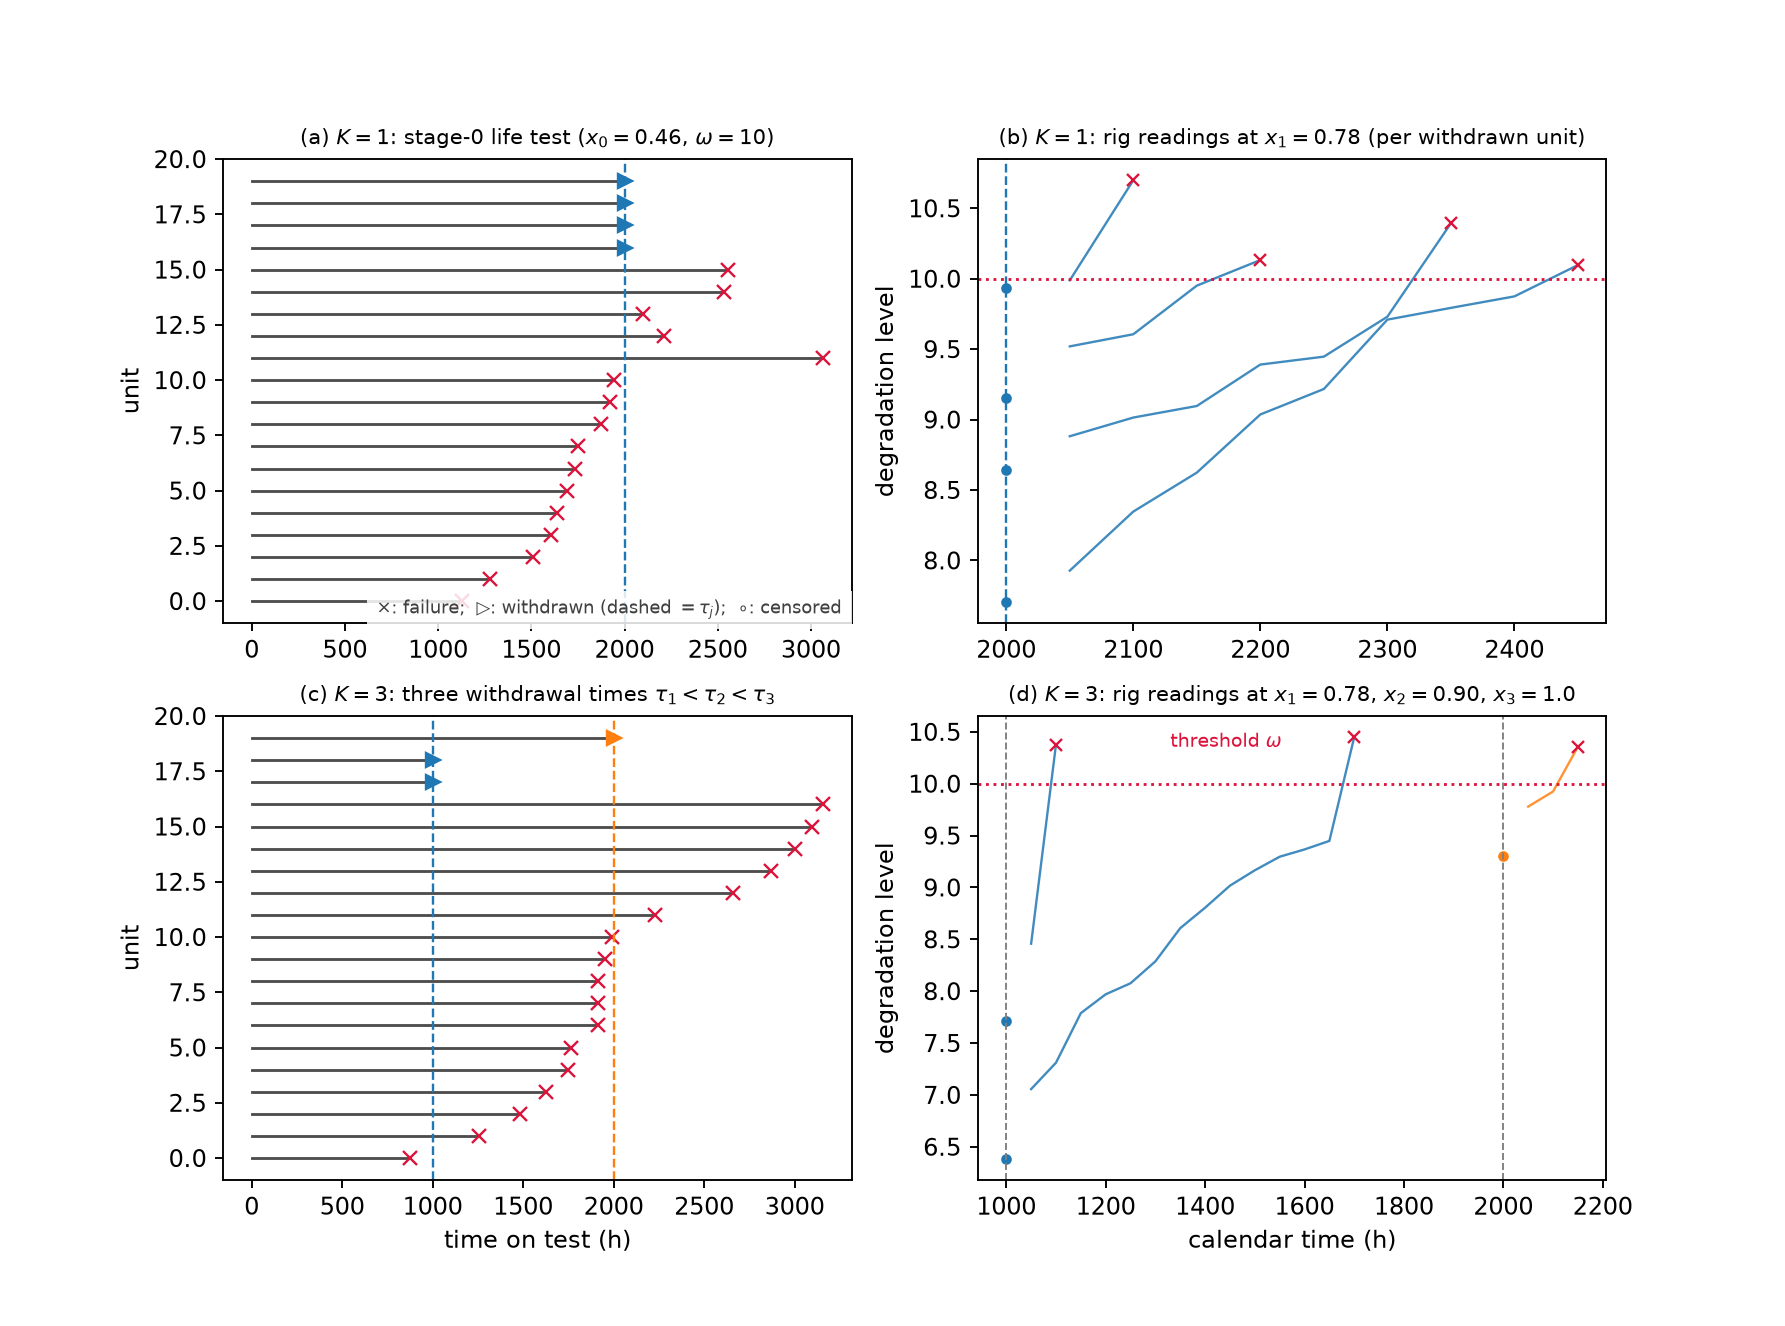
\includegraphics[width=.98\linewidth]{../results/fig_scheme.png}
\caption{Simulated \SLTD{} worlds ($n=20$, $x_0=0.46$, $\omega=10$, $\tmax=5000$ h, readings
every 50 h; true $\theta$ of Section~\ref{sec:case}). Panels (a) and (b) show the $K{=}1$
case: the stage-0 life test, the withdrawal of half the survivors at $\tau_1=2000$ h, and the
rig readings at $x_1=0.78$ (baselines as dots, crossings as $\times$). Panels (c) and (d)
show $K{=}3$: withdrawals at $\tau=(1000,2000,3500)$ h with $\pi=(0.15,0.20,0.25)$ into rigs
at $x=(0.78,0.90,1.0)$.}
\label{fig:scheme}
\end{figure}

\subsection{Multi-stage extension}\label{sec:kstage}

The single change point generalizes to $K$ withdrawal times in the obvious way, yielding a
\emph{k-stage} \SLTD{} that parallels the $k$-step stage life testing of
\citet{LaumenCramer2021}. Let $\tau_1<\dots<\tau_K<\tmax$ be prefixed change times with
withdrawal proportions $\pi_1,\dots,\pi_K$ and rig stresses $x_1,\dots,x_K$ (all exceeding
$x_0$). At $\tau_j$, a randomized subset of $\lfloor\pi_j\cdot(\text{survivors on test})\rfloor$
units is withdrawn to an instrumented rig at stress $x_j$, where a baseline reading and the
periodic readings are taken as before; the units still on test after $\tau_K$ remain on stage
$s_0$ until failure or $\tmax$. Randomized withdrawal at \emph{every} stage is ignorable, so
Lemma~\ref{lem:block} persists verbatim: conditional on the withdrawal history, the stage-$0$
failure/censoring records and the per-cohort baseline-plus-increment records are independent
with their ordinary laws, and the log-likelihood is
\begin{equation}\label{eq:ellk}
\begin{split}
\ell ={}&\sum_{i\in\text{failures}}\ln f_{x_0}(t_i)\;+\;n_{\mathrm{cens}}\ln\bar F_{x_0}(\tmax)
\;+\;\sum_{j=1}^{K}\sum_{k\in\text{cohort }j}
\ln f_{\mathrm{IG}}\big(b_k;\,a_{x_0}(\tau_j),\,b_{x_0}(\tau_j)\big)\\
&+\sum_{j=1}^{K}\sum_{k\in\text{cohort }j}\sum_{l}
\ln f_{\mathrm{IG}}\big(\Delta_{kl};\ \mu_{x_j}\Delta\Lambda_{kl},\ \lambda\Delta\Lambda_{kl}^{2}\big),
\end{split}
\end{equation}
with the virtual ages of cohort $j$ computed at stress $x_j$. Note that no explicit survival
term $\ln\bar F_{x_0}(\tau_j)$ appears for withdrawn units: the level density at $\tau_j$
restricted to $(0,\omega)$ has total mass $\bar F_{x_0}(\tau_j)$, so the baseline density
itself carries the stage-$0$ survival information of the withdrawn unit. $K=1$ recovers
Section~\ref{sec:scheme}; $K\ge2$ spreads the withdrawal over time, which Section
\ref{sec:simk} shows to hedge against the design-collapse mechanism of
Section~\ref{sec:sens} and to improve precision at a matched number of recycled units
(Figure~\ref{fig:scheme}(c)--(d)).

\section{Likelihood and estimation}\label{sec:lik}

\subsection{Ignorable withdrawal and block independence}

\begin{lemma}\label{lem:block}
Conditionally on $D_1=d_1$, the pre-$\tau_1$ failure times, the post-$\tau_1$ failure/censoring
data of the stayers, and the per-unit baseline-plus-increment data of the withdrawn units are
independent, with their ordinary (unconditional) laws. In particular, the likelihood is the
product of the corresponding densities, and no combinatorial factor depending on $\theta$
appears.
\end{lemma}

\begin{proof}
The withdrawal at $\tau_1$ selects uniformly among survivors, independently of degradation
levels; the selection mechanism is therefore ignorable (missing at random), and each unit's
record is a draw from its model density on its observation space (failure density $f_{x_0}$ on
$(0,\tau_1]$; stayer failure density on $(\tau_1,\tmax]$ or point mass $S_{x_0}(\tmax)$;
withdrawn joint density over level and increments on $\{b<\omega\}$). The product form follows;
this is the \SLTD{} analogue of Lemma~3.3 of \citet{LaumenCramer2019}.
\end{proof}

Writing $\bar F_x=1-F_x$, the common stage-0 block of all schemes is
\begin{equation}\label{eq:fail}
\ell_{\mathrm{fail}}=\sum_{i\le d_1}\ln f_{x_0}(t_i)
+\Bigg[\;\sum_{\text{stayers}}\!\!\Big(\ind{t_i\le\tmax}\ln f_{x_0}(t_i)
+\ind{t_i>\tmax}\ln \bar F_{x_0}(\tmax)\Big)\Bigg],
\end{equation}
and the withdrawn-arm contributions are
\begin{align}
\text{(a)}\quad & \ell_{\mathrm{w}}=r_1^{*}\ln \bar F_{x_0}(\tau_1); \label{eq:ella}\\[2pt]
\text{(b)}\quad & \ell_{\mathrm{w}}=\sum_{k=1}^{r_1^{*}}
\begin{cases}
\ln m_f(u_k), & \text{unit $k$ fails at offset } u_k\le \tmax-\tau_1,\\[2pt]
\ln m_s, & \text{unit $k$ censored at } \tmax,
\end{cases}\label{eq:ellb}\\
&\qquad m_f(u)=\int_0^{\omega}\! f_{\mathrm{IG}}\big(b;\,a_{x_0}(\tau_1),b_{x_0}(\tau_1)\big)\,
g(u\mid b)\,db, \notag\\
&\qquad m_s=\int_0^{\omega}\! f_{\mathrm{IG}}\big(b;\,a_{x_0}(\tau_1),b_{x_0}(\tau_1)\big)
\big(1-G(\tmax-\tau_1\mid b)\big)\,db; \notag\\[2pt]
\text{(c)}\quad & \ell_{\mathrm{w}}=\sum_{k=1}^{r_1^{*}}
\Bigg[\ln f_{\mathrm{IG}}\big(b_k;\,a_{x_0}(\tau_1),b_{x_0}(\tau_1)\big)
+\sum_{j}\ln f_{\mathrm{IG}}\big(\Delta_{kj};\ \mu_{x_1}\Delta\Lambda_{kj},\ \lambda\Delta\Lambda_{kj}^{2}\big)\Bigg],
\label{eq:ellc}
\end{align}
where in \eqref{eq:ellc} $b_k$ is the baseline reading, $\Delta_{kj}$ the observed increments,
$\Delta\Lambda_{kj}=(w_k+u_j)^{q}-(w_k+u_{j-1})^{q}$ with $w_k=w(b_k)$ and $u_0=0$, and the sum
over $j$ extends over the readings taken (including the crossing reading, which is an ordinary
IG observation because the level is what is read). Scheme~(c) is fully closed-form; the
integrals in \eqref{eq:ellb} are one-dimensional and computed by Gauss--Legendre quadrature.

\subsection{Estimation and asymptotic inference}

The maximum likelihood estimator $\hat\theta$ of $\theta=(\alpha_0,\alpha_1,\lambda,q)$ is
obtained by multi-start Nelder--Mead search in the unconstrained parameterization
$(\alpha_0,\alpha_1,\ln\lambda,\ln q)$, with the covariance from the numerically inverted
observed information. Delta-method inference for the use-condition quantile uses the gradient
of $\ln\xi_p(0)$ from \eqref{eq:xi}; we report Wald intervals for $\ln\hat\xi_p$, whose error is
naturally interpreted as a relative error of $\hat\xi_p$.

\subsection{Variant without baseline reading, and an EM algorithm}\label{sec:em}

If no reading is taken at the switch, the level $b_k$ is latent with prior
$f_{\mathrm{IG}}(b;\,a_{x_0}(\tau_1),b_{x_0}(\tau_1))$ restricted to $b\in(0,\omega)$, and the
observed likelihood of unit $k$'s readings is
\begin{equation}\label{eq:ellB}
L_k=\int_0^{\omega} f_{\mathrm{IG}}(b)\prod_{j}
f_{\mathrm{IG}}\big(\Delta_{kj}\mid b\big)\,db,
\end{equation}
where the first increment is $\ell_{k1}-b$ (level at first reading minus latent baseline) and
later increments are observed differences; nodes with $b\ge \ell_{k1}$ contribute zero density
because IG paths are monotone, so the integral automatically restricts the latent support. An EM
view treats $b$ as missing data: the E-step conditional density is proportional to the integrand
of \eqref{eq:ellB} (no closed form; evaluated by quadrature), and the M-step maximizes the
expected complete-data log-likelihood numerically ($\theta$ enters the increment means through
the virtual age $w(b;\theta)$, so no closed-form M-step exists). In our implementation the
equivalent direct maximization of the quadrature-approximated marginal \eqref{eq:ellB} is used;
simulation shows it remains consistent with a modest precision loss relative to the
baseline-reading variant (Section~\ref{sec:sim}).

\subsection{Identifiability and the role of the withdrawn units}\label{sec:ident}

\begin{proposition}\label{prop:ident}
Under scheme~(a), all observed data carry the single stress $x_0$ only. The likelihood then
depends on $\theta$ solely through the first-passage law $F_{x_0}$, which identifies at most
three functionals of the four parameters; the pair $(\alpha_0,\alpha_1)$ is not separable and
$\xi_p(0)$ is not identified.
\end{proposition}

The proof is immediate: $f_{x_0}$, $\bar F_{x_0}(\tau_1)$ and $\bar F_{x_0}(\tmax)$ involve
$\theta$ only through $(\mu_{x_0},\lambda,q)$, and $\xi_p(0)$ requires $\mu_{0}=e^{\alpha_0}$
and $\mu_{x_0}=e^{\alpha_0+\alpha_1 x_0}$ separately. Scheme (b) and \SLTD{} restore
identifiability through the stage-$1$ arm. The practical force of Proposition~\ref{prop:ident}
is illustrated by profile likelihood in Section~\ref{sec:sim} (Figure~\ref{fig:ridge}): with
zero stage-0 failures, the approximate $15\%$ profile-likelihood region of scheme~(a) contains
$(\alpha_0,\alpha_1)$ pairs whose implied $\xi_{0.1}(0)$ spans a factor $e^{13.1}$, versus
$e^{1.1}$ for \SLTD{} on the same data.

\section{Planning information and V-optimal designs}\label{sec:design}

\subsection{Expected information of an \SLTD{} plan}

For planning we need the Fisher information of the design rather than of a realization.
Let $\mathcal{D}=(x_0,\tau_1,\pi_1,x_1,u_1,\dots,u_L)$ denote the plan. Per test unit, the
expected information is
\begin{equation}\label{eq:I}
\begin{split}
\mathcal{I}(\theta;\mathcal{D})={}&
\underbrace{\int_0^{\tau_1}\!\! f_{x_0} H_f
+(1-\pi_1)\Big[\int_{\tau_1}^{\tmax}\!\! f_{x_0} H_f+\bar F_{x_0}(\tmax)H_S\Big]}_{\text{stage-0 block}}\\
&+\underbrace{\pi_1\!\int_0^{\omega}\!\! f_B(b)\Big[H_b(b)+\sum_{j=1}^{L}\ind{\text{alive}_j(b)}
J_j(b)^{\!\top} W_j(b)\, J_j(b)\Big]db}_{\text{withdrawn block}}
\end{split}
\end{equation}
where $H_f(t)=-\ddot{\ell}_\theta\ln f_{x_0}(t)$ and analogously $H_S$, $H_b$ for the censoring
term and the baseline reading ($f_B$ the level density at $\tau_1$), and for the $j$-th
continuation increment with mean/shape $(a_j,s_j)$, $W_j=\mathrm{diag}(s_j/a_j^{3},\,1/2s_j^{2})$
is the IG$(a,s)$ information and $J_j=\partial(a_j,s_j)/\partial\theta$ (the second-derivative
term vanishes in expectation because the IG score has zero mean; Appendix~\ref{app:info}).
A standard planning approximation evaluates \eqref{eq:I} with all $L$ readings. Because IG paths
cross $\omega$ in finite time, withdrawn units with fast degradation stop contributing readings;
we therefore weight the $j$-th increment by
\begin{equation}\label{eq:alive}
P(\text{alive}_j\mid b)=1-G(u_{j-1}\mid b),
\end{equation}
the probability that the unit is still operational at the previous reading. This refinement is
quantitatively important: in our moderate scenario it changes the predicted information by tens
of percent (Section~\ref{sec:sim}) and its predictions then match the simulated variances
closely (Table~\ref{tab:avarcheck}). The V-optimality criterion is
\begin{equation}\label{eq:V}
\Asvar\{\ln\hat\xi_p(0)\}=\nabla_\theta^{\top}\ln\xi_p(0)\;\big(n\,\mathcal{I}\big)^{-1}\;\nabla_\theta\ln\xi_p(0),
\end{equation}
with $\nabla\ln\xi_p$ from \eqref{eq:xi}.

\subsection{Constrained and unconstrained optima, and the price of sequentiality}

The plan is optimized over $(x_0,\tau_1,\pi_1,x_1,\text{step},n)$ under a budget
\begin{equation}\label{eq:budget}
n\big(C_b+C_{\mathrm{mea}}\,\pi_1\bar F_{x_0}(\tau_1)\,L\big)\;\le\;\text{budget},\qquad n\le n_{\max},
\end{equation}
with unit cost $C_b$ and per-reading cost $C_{\mathrm{mea}}$ \citep[cf.][]{Ma2021}. As the
unconstrained benchmark we optimize a \emph{parallel} two-level constant-stress ADT ($n_1$
units at $x_a$, $n_2$ at $x_b$, all measured over $(0,\tmax]$) under the same budget. The
benchmark represents a world in which any unit can be instrumented from the start; the \SLTD{}
optimum represents the constrained world in which the first stage must be a failure-only life
test, as in a sealed chamber or a mandated certification run. Their ratio quantifies the
\emph{price of the stage-wise constraint}. Table~\ref{tab:design} reports both optima for the connector
case ($C_b=\$200$, $C_{\mathrm{mea}}=\$5$, budget $\$6000$, $n_{\max}=30$, $\tmax=5000$ h): the
constrained optimum places stage~0 at the lowest grid stress ($x_0=0.10$, about $45^\circ$C on
the Arrhenius scale), withdraws $\pi_1=0.90$ of survivors at $\tau_1=1750$ h into a rig at
$x_1=0.85$ (about $89^\circ$C) with readings every 150 h, $n=20$, achieving
$\Asvar=0.036$ ($\mathrm{sd}=e^{0.19}$, that is, $\pm21\%$ on the quantile); the
unconstrained parallel ADT concentrates units at $x_a=0$, the use condition itself, and
reaches $\Asvar=0.0066$. The price of sequentiality is thus a factor of about $5.5$ in
asymptotic variance (about $2.3$ in standard deviation) for this product and horizon, because
the connector's degradation is measurable at low stress within $\tmax$. This echoes the
optimal low-stress plans of \citet{Ma2021} and \citet{Ye2014}. The structure of the optimum
is informative in its own right: the criterion pushes the stage-0 stress down and the
withdrawal early because, at least for this product, the recycled degradation information
matters more than the stage-0 failure information, and a low $x_0$ maximizes the surviving arm
at almost no cost in reading time. Under the sequential constraint the life-test stage acts
chiefly as an ageing phase whose surviving units are the real measurement resource.
Figure~\ref{fig:design} maps the criterion over $(x_0,\tau_1)$ at the optimal $\pi_1$, rig
stress and cadence: the optimum sits in a broad low-stress basin, far from the survival cliff
$F_{x_0}(\tau_1)\to1$ (red contour) that marks the collapsed designs of
Section~\ref{sec:sens}.

\begin{figure}[t]
\centering
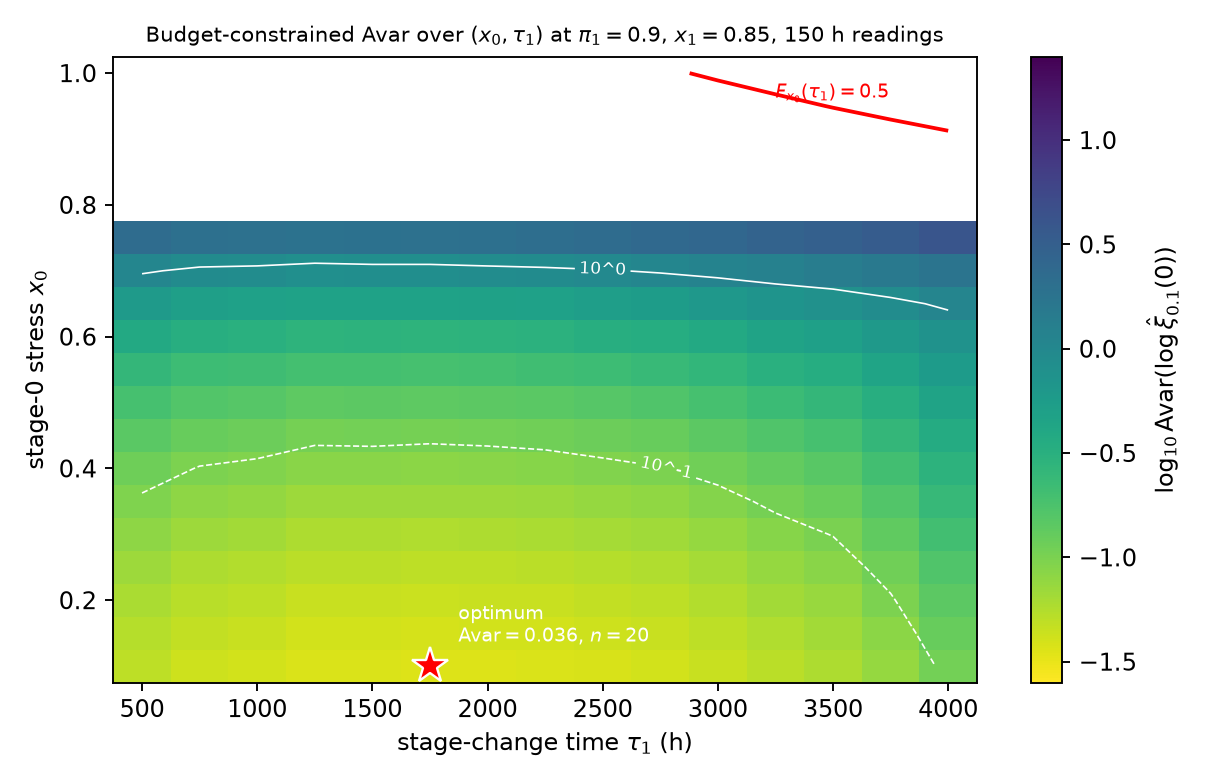
\includegraphics[width=.8\linewidth]{../results/fig_design_landscape.png}
\caption{Budget-constrained $\Asvar$ of $\ln\hat\xi_{0.1}(0)$ over $(x_0,\tau_1)$ at
$\pi_1=0.9$, rig stress $x_1=0.85$, 150 h readings; $n$ re-derived from the budget at each
point (white region: $x_0$ must lie below the rig stress). The star marks the constrained
optimum; the red contour is the survival cliff $F_{x_0}(\tau_1)=0.5$ of
Section~\ref{sec:sens} (the $0.95$ contour lies outside this slice).}
\label{fig:design}
\end{figure} When use-condition degradation is too
slow to read within the horizon (or when the life test is mandated), the constrained \SLTD{}
plan is the relevant optimum, and Table~\ref{tab:l9plan} shows it is robust: under an
$L_9(3^4)$ array of $\pm10\%$ planning errors in $(\alpha_0,\alpha_1,\lambda,q)$, all nine
re-optimized plans remain within a factor $1.4$ of the base optimum ($\Asvar\le0.052$ at the
true parameters), with the qualitative features (low $x_0$, large $\pi_1$, 150 h readings)
entirely stable.

\begin{table}[t]
\centering\small
\caption{Constrained-optimal \SLTD{} plan versus the unconstrained parallel two-level ADT at
the same budget ($C_b=\$200$ per unit, $C_{\mathrm{mea}}=\$5$ per reading, budget $\$6{,}000$,
$n_{\max}=30$, $\tmax=5000$ h; connector parameters; $\Asvar$ of $\ln\hat\xi_{0.1}(0)$).}
\label{tab:design}
\begin{tabular}{lrrrrrrr}
\toprule
Design & $x_0$/ $x_a$ & $\tau_1$ & $\pi_1$ & $x_1$/ $x_b$ & step & $n$ & $\Asvar$ \\
constrained SLT-D & 0.10 & 1750 & 0.90 & 0.85 & 150 & 20 & 0.0362 \\
parallel two-level ADT & 0.00 & -- & -- & 0.20 & 150 & 16 & 0.0066 \\
\bottomrule
\end{tabular}

\end{table}

\begin{table}[t]
\centering\small
\caption{Robustness of the optimal \SLTD{} plan: $L_9(3^4)$ array of $\pm10\%$ planning-value
errors in $(\alpha_0,\alpha_1,\lambda,q)$; each row re-optimizes the plan at the perturbed
planning values and evaluates $\Asvar$ at the true parameters (base optimum: $0.036$).}
\label{tab:l9plan}
\begin{tabular}{rrrrrrrr}
\toprule
$\epsilon_{\alpha_0}$ & $\epsilon_{\alpha_1}$ & $\epsilon_{\lambda}$ & $\epsilon_q$ & $\tau_1$ & $\pi_1$ & step & $\Asvar$ at truth \\
-10\% & -10\% & -10\% & -10\% & 2000 & 0.90 & 150 & 0.0391 \\
-10\% & +0\% & +0\% & +0\% & 2250 & 0.90 & 150 & 0.0370 \\
-10\% & +10\% & +10\% & +10\% & 3250 & 0.90 & 150 & 0.0518 \\
+0\% & -10\% & +0\% & +10\% & 2000 & 0.90 & 150 & 0.0364 \\
+0\% & +0\% & +10\% & -10\% & 1250 & 0.90 & 150 & 0.0369 \\
+0\% & +10\% & -10\% & +0\% & 2250 & 0.90 & 150 & 0.0370 \\
+10\% & -10\% & +10\% & +0\% & 1250 & 0.90 & 150 & 0.0369 \\
+10\% & +0\% & -10\% & +10\% & 2000 & 0.90 & 150 & 0.0364 \\
+10\% & +10\% & +0\% & -10\% & 1750 & 0.90 & 150 & 0.0362 \\
\bottomrule
\end{tabular}

\end{table}

\subsection{Bayesian planning under parameter uncertainty}\label{sec:bayes}

The $L_9$ analysis treats planning errors one scenario at a time. An alternative is to
average the criterion itself over a prior distribution for $\theta$ \citep[cf.][]{Li2017}. We
take the prior to be what a pilot study of the case-study product would supply: a multivariate
normal on $z=(\alpha_0,\alpha_1,\ln\lambda,\ln q)$ centered at the pilot MLE with covariance
$\kappa$ times the inverse observed information of the pilot likelihood ($\kappa=1$ for the
18-unit connector pilot; $\kappa=4$ emulates a pilot a quarter as informative). The resulting
marginal prior standard deviations are $0.19$, $0.18$, $0.31$, and $0.04$. Nonlinearity $q$ is
pinned down tightly by the within-unit reading trajectories; the stress-acceleration pair and
$\lambda$ remain comparatively uncertain. The Bayesian
V-optimal plan minimizes the pre-posterior criterion
\begin{equation}\label{eq:bayes}
J(\mathcal{D})\;=\;\E_{\theta\sim\text{prior}}\big[\Asvar\{\ln\hat\xi_p(0);\,\theta,\mathcal{D}\}\big],
\end{equation}
evaluated by averaging \eqref{eq:V} over $400$ prior draws, with the design variables and the
budget-feasible $n$ chosen exactly as in Section~\ref{sec:design} (the budget is committed at
the planning values; only the criterion is averaged).

Table~\ref{tab:bayes} compares the Bayesian-optimal plan with the plug-in plan optimized at
the prior mean. At both prior scales the two criteria select the same plan, namely the
constrained optimum of Table~\ref{tab:design}, so the Bayesian criterion serves here as a
robustness certificate rather than a correction. Under the full pilot the prior-expected
criterion is $J=0.037$ with 90th percentile $0.041$; with a pilot a quarter as informative
($\kappa=4$) it is $J=0.038$ with $0.047$ (Figure~\ref{fig:bayes}b). All of these are close
to the plug-in value of $0.036$, so the plan's precision is insensitive to plausible pilot
errors. Why averaging leaves the optimum in place can be read off Figure~\ref{fig:bayes}(a):
at the constrained optimum the stage-$0$ stress is low ($x_0=0.10$) and
$F_{x_0}(\tau_1)\approx0$, the recycled arm is guaranteed for every prior draw, the collapse
boundary sits many prior standard deviations away, and the $\Asvar$ surface is nearly
symmetric in the uncertain directions. The expectation is then well approximated by its value
at the mean. The Bayesian correction becomes first-order only when the prior mass approaches
the survival cliff of Section~\ref{sec:sens}, that is, in regimes with $F_{x_0}(\tau_1)$ near
$0.5$ where collapse draws dominate the expectation and pull the optimum toward earlier
withdrawal and lower $x_0$; in those regimes the multi-stage withdrawal of
Section~\ref{sec:simk} is the structural safeguard.

\begin{figure}[t]
\centering
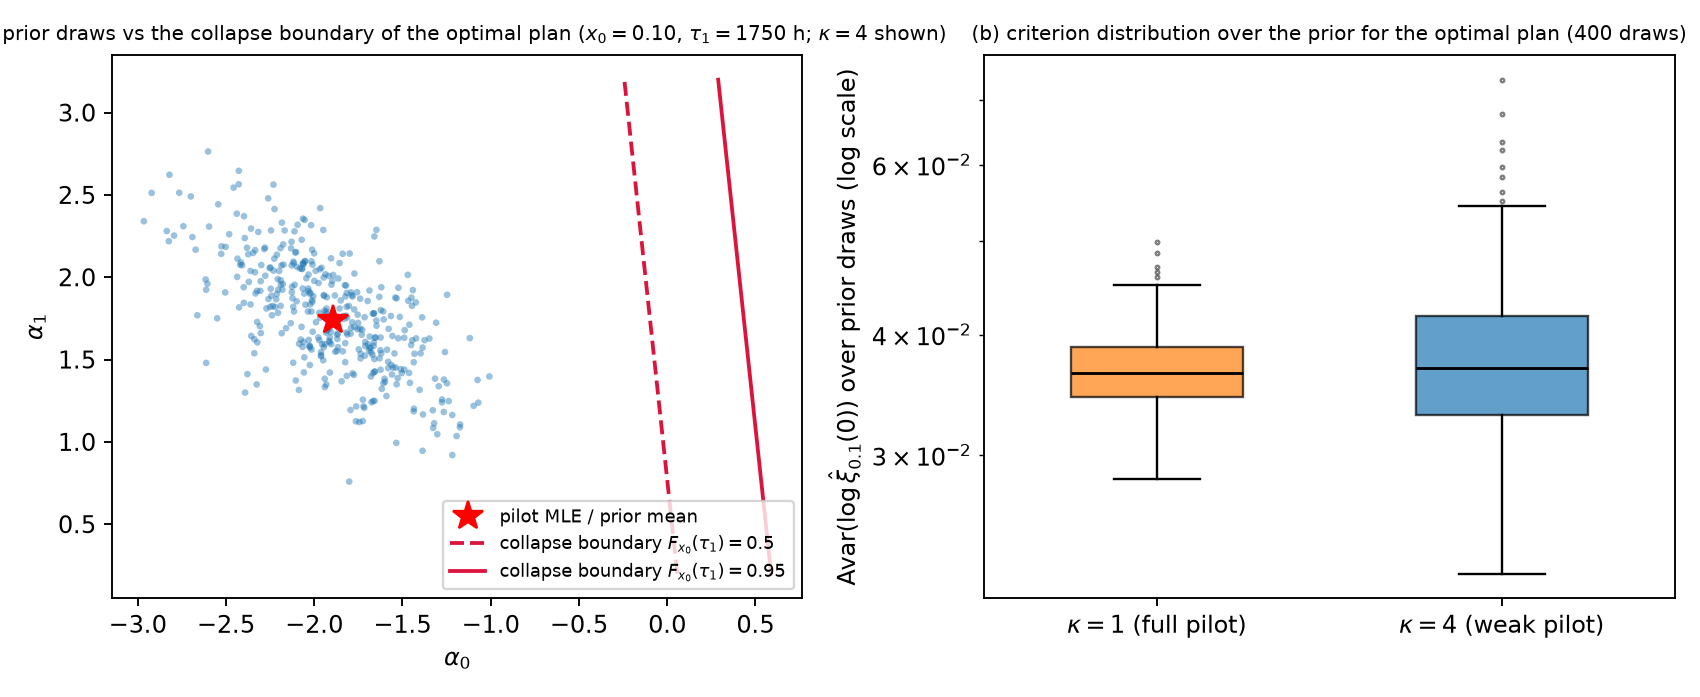
\includegraphics[width=.95\linewidth]{../results/fig_bayes_prior.png}
\caption{Bayesian planning diagnostics. (a) Prior draws ($\kappa=4$) in the
$(\alpha_0,\alpha_1)$ plane against the collapse boundaries
$F_{x_0}(\tau_1)=0.5$/$0.95$ of the optimal plan: the prior mass lies far from the cliff, so
averaging over the prior cannot move the optimum. (b) Distribution of
$\Asvar(\ln\hat\xi_{0.1}(0))$ over $400$ prior draws for the optimal plan under the full
($\kappa=1$) and a quarter-as-informative ($\kappa=4$) pilot.}
\label{fig:bayes}
\end{figure}

\begin{table}[t]
\centering\small
\caption{Bayesian versus plug-in V-optimal \SLTD{} plans under pilot-informed priors
($400$ prior draws; budget and constraints as in Table~\ref{tab:design}). $\kappa$ scales the
pilot covariance ($\kappa=1$: the 18-unit pilot). $J$: prior-expected $\Asvar$ of
$\ln\hat\xi_{0.1}(0)$; $J_{90}$: its 90th percentile over the prior.}
\label{tab:bayes}
\begin{tabular}{llrrrrrrrrr}
\toprule
Prior & Plan & $x_0$ & $\tau_1$ & $\pi_1$ & $x_1$ & step & $n$ & $J$ & $J_{90}$ & $\Asvar$ at mean \\
$\kappa{=}1$ & Bayesian & 0.10 & 1750 & 0.9 & 0.85 & 150 & 20 & 0.0368 & 0.0411 & 0.0362 \\
$\kappa{=}1$ & plug-in & 0.10 & 1750 & 0.9 & 0.85 & 150 & 20 & 0.0368 & 0.0411 & 0.0362 \\
\addlinespace
$\kappa{=}4$ & Bayesian & 0.10 & 1750 & 0.9 & 0.85 & 150 & 20 & 0.0380 & 0.0472 & 0.0362 \\
$\kappa{=}4$ & plug-in & 0.10 & 1750 & 0.9 & 0.85 & 150 & 20 & 0.0380 & 0.0472 & 0.0362 \\
\addlinespace
\bottomrule
\end{tabular}

\end{table}

\section{Simulation study}\label{sec:sim}

\subsection{Design of the experiments}

True parameters are our fit of the connector data (Section~\ref{sec:case}),
$\theta=(-1.8944,\,1.7377,\,0.6285,\,0.4491)$. Three scenarios (Table~\ref{tab:scen}) span the
reliability range: S1 (connector-like: $x_0=0.78$ [$85^\circ$C], $x_1=1.0$ [$100^\circ$C],
$\omega=30$, $n=20$) with essentially no stage-0 failures; S2 (moderate: $x_0=0.46$
[$65^\circ$C], $x_1=0.78$, $\omega=10$, $n=20$) with rich failure data; S3 (severe: $x_0=0.46$,
$x_1=0.78$, $\omega=30$, $n=30$) with zero failures anywhere on stage~0. All plans use
$\tau_1=2000$ h, $\tmax=5000$ h, $\pi_1=0.5$ (S2 additionally sweeps $\pi_1\in\{0.25,0.5,0.75\}$);
readings every 150 h (S1, S3) or 50 h (S2). Each cell aggregates $1000$ independent worlds; the
three schemes are evaluated on common random numbers. Estimand: $\ln\xi_{0.1}(0)$. Multi-start
maximization is initialized from jittered planning values plus one generic start; fits whose
numerical information is not positive definite are flagged.

\begin{table}[t]
\centering\small
\caption{Simulation scenarios. Stresses standardized by the Arrhenius rule
$x=(1/s_0-1/s)/(1/s_0-1/s_H)$, $s_0=313.15$ K ($40^\circ$C), $s_H=373.15$ K ($100^\circ$C).}
\label{tab:scen}
\begin{tabular}{lcccccc}
\toprule
& $x_0$ & $x_1$ & $\omega$ & $n$ & readings & $F_{x_0}(\tau_1)$\\
\midrule
S1 (connector-like) & 0.78 & 1.00 & 30 & 20 & every 150 h & $\approx0.001$\\
S2 (moderate)       & 0.46 & 0.78 & 10 & 20 & every 50 h  & $\approx0.55$\\
S3 (severe)         & 0.46 & 0.78 & 30 & 30 & every 150 h & $\approx0$\\
\bottomrule
\end{tabular}
\end{table}

\subsection{Information hierarchy}

Table~\ref{tab:hierarchy}, Figures~\ref{fig:rmse} and \ref{fig:errors} give the
headline results; errors are on the
log scale, so RMSE $=0.5$ means a typical factor-$e^{0.5}\approx1.6$ error of the quantile.
Three findings stand out. First, scheme~(a) cannot extrapolate to the use condition in any
scenario (RMSE $23$ to $54$). By Proposition~\ref{prop:ident} its single-stress likelihood
leaves $(\alpha_0,\alpha_1)$ unresolved, and the wild point estimates (positive bias up to
$+33$ in log) simply sit on a flat ridge of the likelihood. The apparently tame RMSE of
scheme~(a) in S3 is an artefact of truth-anchored optimizer starts on that ridge; its
numerical information is never positive definite. Second, \SLTD{} dominates SLT failure
re-testing everywhere: RMSE $0.84$ against $32.9$ in S1 ($39\times$), $0.53$ against $1.82$
in S2 ($3.4\times$), $0.41$ against $8.95$ in S3 ($22\times$). The mechanism shows up in the
tails and in the inference. The continuation failure times of scheme~(b) carry little
information about $(\lambda,q)$: its 90th-percentile absolute error reaches $11.4$ in S3
(versus $0.68$ for \SLTD{}), its observed information is positive definite in only
$79$ to $93\%$ of fits (versus $99$ to $100\%$ for \SLTD{}), the median standard error in S3
is of order $3\times10^{4}$ where the Hessian is near-singular, and the Wald intervals
undercover accordingly ($78\%$ in S3). The intervals of \SLTD{}, by contrast, are calibrated:
coverage between $88$ and $95\%$ across scenarios, with median standard errors of $0.42$ to
$0.82$ that match the empirical RMSE. Third, the gain is largest exactly where accelerated
testing matters most. In the failure-free scenarios S1 and S3 the life test produces almost no
failures, yet \SLTD{} still estimates the use-condition quantile to within a factor of about
$1.5$ ($e^{0.41}$, median error).

\begin{figure}[t]
\centering
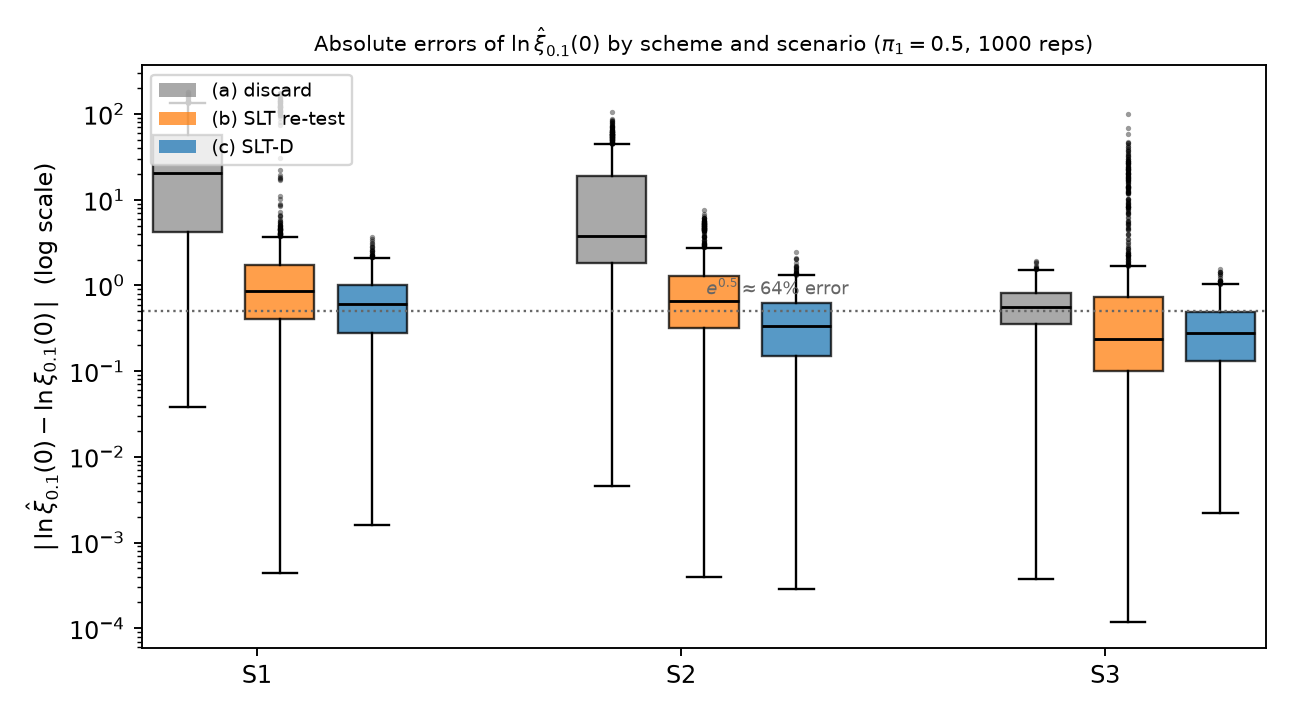
\includegraphics[width=.9\linewidth]{../results/fig_error_dist.png}
\caption{Distributions of the absolute error of $\ln\hat\xi_{0.1}(0)$ (log scale;
$\pi_1=0.5$, 1000 replications). \SLTD{} concentrates near the $e^{0.5}\approx64\%$ level
or below, whereas scheme~(b) develops heavy tails (note the outlier strings in S1/S3) and
scheme~(a) is off by orders of magnitude.}
\label{fig:errors}
\end{figure}

\begin{table}[t]
\centering\small
\caption{Information hierarchy at $\pi_1=0.5$ (1000 replications). Bias, RMSE, median and 90th
percentile of the absolute error of $\ln\hat\xi_{0.1}(0)$. Scheme (a): see text regarding S3.}
\label{tab:hierarchy}
\begin{tabular}{llrrrrrr}
\toprule
Scenario & Scheme & $\bar d_1$ & $\bar r_1^*$ & Bias & RMSE & MdAE & p90AE \\
S1 (connector-like) & (a) & 0.02 & 9.98 & 33.435 & 52.855 & 20.587 & 93.500 \\
S1 (connector-like) & (b) & 0.02 & 9.98 & 9.255 & 34.409 & 0.873 & 4.745 \\
S1 (connector-like) & (c) & 0.02 & 9.98 & 0.094 & 0.920 & 0.609 & 1.478 \\
\addlinespace
S2 (moderate) & (a) & 10.60 & 4.46 & 11.571 & 23.283 & 3.810 & 44.466 \\
S2 (moderate) & (b) & 10.60 & 4.46 & 0.438 & 1.749 & 0.654 & 2.855 \\
S2 (moderate) & (c) & 10.60 & 4.46 & 0.028 & 0.550 & 0.335 & 0.879 \\
\addlinespace
S3 (severe) & (a) & 0.00 & 15.00 & 0.589 & 0.681 & 0.562 & 1.027 \\
S3 (severe) & (b) & 0.00 & 15.00 & 2.725 & 8.875 & 0.241 & 10.434 \\
S3 (severe) & (c) & 0.00 & 15.00 & 0.030 & 0.441 & 0.279 & 0.737 \\
\bottomrule
\end{tabular}

\end{table}

\begin{figure}[t]
\centering
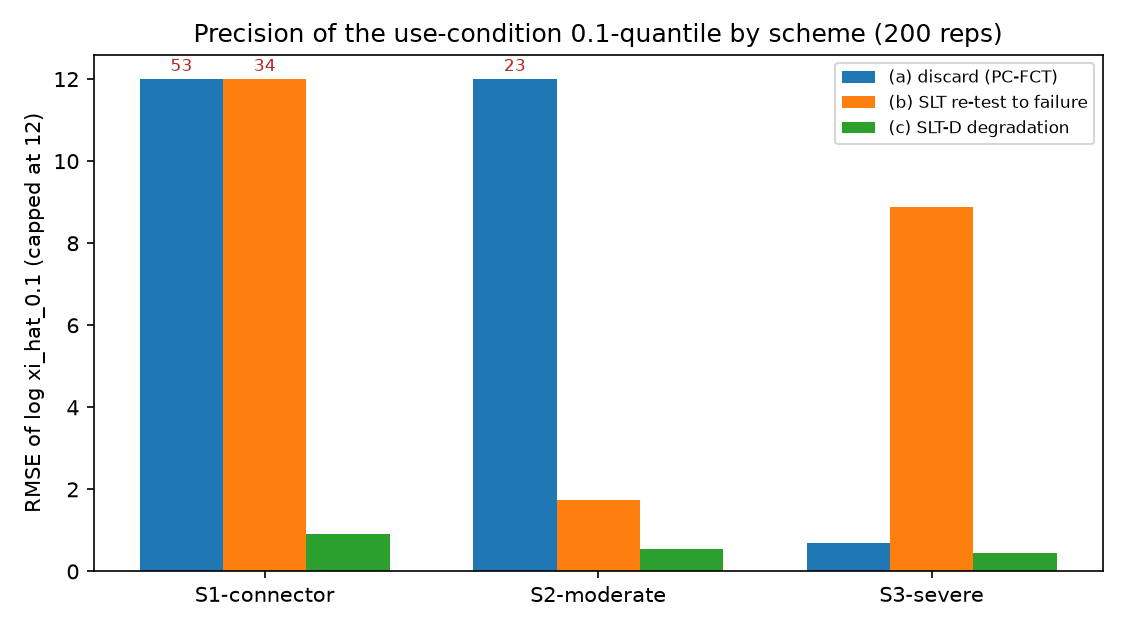
\includegraphics[width=.95\linewidth]{../results/fig1_rmse_by_scheme.png}
\caption{RMSE of $\ln\hat\xi_{0.1}(0)$ by scheme and scenario (bars capped at 12 for display;
printed values above capped bars). \SLTD{} (scheme c) dominates throughout.}
\label{fig:rmse}
\end{figure}

\subsection{Withdrawal fraction}

Table~\ref{tab:pisweep} sweeps $\pi_1$ in S2. \SLTD{} improves monotonically in $\pi_1$
(RMSE $0.95\to0.53\to0.46$ for $\pi_1=0.25,0.5,0.75$): within the fixed budget of units, the
more survivors are recycled into measurement, the better, as long as stage~0 retains its
(censoring) information. Scheme~(b) improves similarly but remains $2$--$3.8\times$ worse at
each $\pi_1$; even with only $\pi_1=0.25$ withdrawn, \SLTD{} is at least as good as scheme~(b)
at $\pi_1=0.75$. Figure~\ref{fig:pisweep} visualizes the sweep.

\begin{figure}[t]
\centering
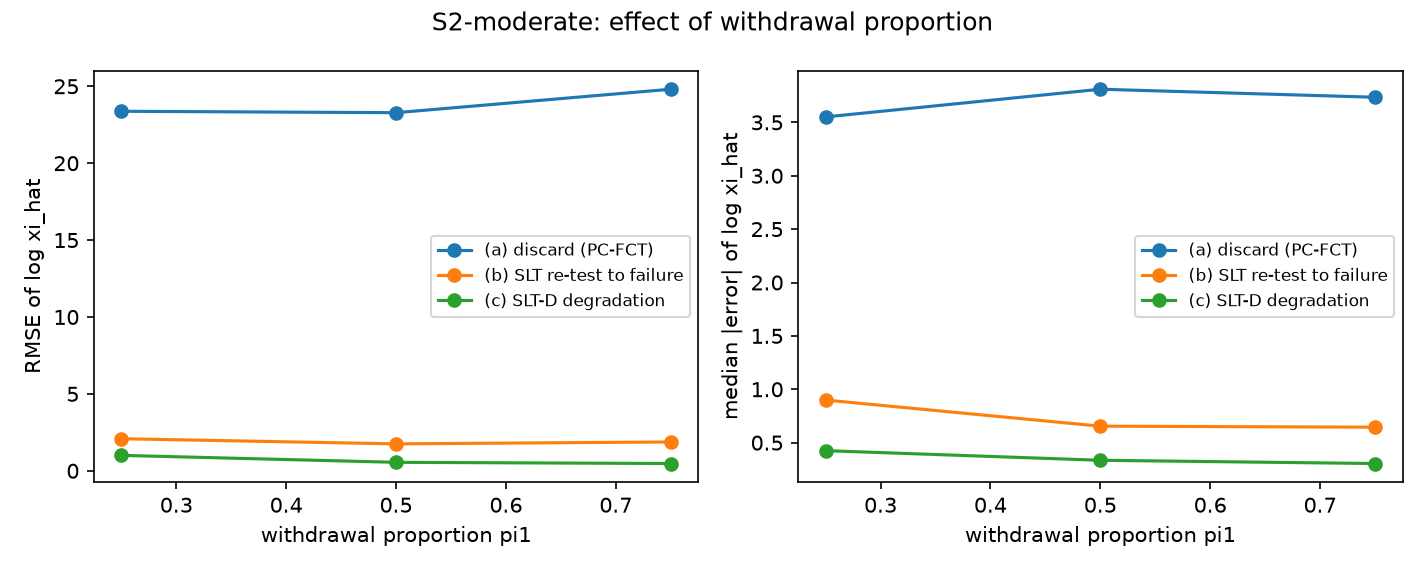
\includegraphics[width=.95\linewidth]{../results/fig2_pi_sweep.png}
\caption{Effect of the withdrawal proportion $\pi_1$ in scenario S2 (schemes (b) and (c);
1000 replications).}
\label{fig:pisweep}
\end{figure}

\begin{table}[t]
\centering\small
\caption{Effect of the withdrawal proportion $\pi_1$ in scenario S2 (1000 replications).
Cov.: empirical coverage (\%) of the 95\% Wald interval.}
\label{tab:pisweep}
\begin{tabular}{crrrrrrr}
\toprule
$\pi_1$ & Scheme & $\bar d_1$ & $\bar r_1^*$ & Bias & RMSE & MdAE & Cov. \\
0.25 & (a) & 10.41 & 2.03 & 11.617 & 23.375 & 3.551 & 100.0 \\
0.25 & (b) & 10.41 & 2.03 & 0.722 & 2.085 & 0.899 & 94.2 \\
0.25 & (c) & 10.41 & 2.03 & 0.282 & 1.002 & 0.425 & 87.8 \\
\addlinespace
0.50 & (a) & 10.60 & 4.46 & 11.571 & 23.283 & 3.810 & 100.0 \\
0.50 & (b) & 10.60 & 4.46 & 0.438 & 1.749 & 0.654 & 92.0 \\
0.50 & (c) & 10.60 & 4.46 & 0.028 & 0.550 & 0.335 & 92.6 \\
\addlinespace
0.75 & (a) & 10.39 & 6.83 & 12.666 & 24.809 & 3.735 & 99.9 \\
0.75 & (b) & 10.39 & 6.83 & 0.522 & 1.874 & 0.645 & 94.1 \\
0.75 & (c) & 10.39 & 6.83 & -0.005 & 0.471 & 0.305 & 95.3 \\
\addlinespace
\bottomrule
\end{tabular}

\end{table}

\subsection{Multi-stage withdrawal}\label{sec:simk}

Table~\ref{tab:kstage} compares $K=1,2,3$ \SLTD{} plans in scenario S2 with $n=20$ units,
$\tmax=5000$ h, readings every 50 h, and expected numbers of withdrawn units matched at
$3.9$--$4.5$: $K{=}1$ withdraws half the survivors at $\tau_1=2000$ h into a $x_1=0.78$ rig;
$K{=}2$ adds a second change at $\tau_2=3000$ h into a $x_2=1.0$ rig ($\pi=(0.30,0.30)$);
$K{=}3$ spreads withdrawal as $(\tau,\pi,x)=(1000,0.15,0.78)$, $(2000,0.20,0.90)$,
$(3500,0.25,1.00)$. Spreading the withdrawal improves precision: the RMSE of
$\ln\hat\xi_{0.1}(0)$ falls from $0.54$ ($K{=}1$) to $0.46$ ($K{=}2$) and $0.42$ ($K{=}3$),
a $22\%$ reduction. Two effects drive this. Earlier cohorts are withdrawn while
$\bar F_{x_0}(\tau)\approx1$ units remain, so the recycled arm stays large; in the language
of Section~\ref{sec:sens}, the plan moves away from the $F_{x_0}(\tau_1)$ cliff (none of the
$K{\ge}2$ replications collapsed, and the design is protected against planning errors that
would empty a single late cohort). In addition, the cohorts observe degradation at two or
three distinct stresses, which separates the acceleration parameters more cleanly. The gain
has a price: with the reading cadence fixed, later-drawn cohorts remain under measurement
longer and the expected total number of readings rises from $14.7$ to about $20$. Normalized
per reading, however, efficiency still improves
(RMSE$\,\times\,\sqrt{\text{readings}}$: $2.07\to2.04\to1.91$), so multi-stage withdrawal
is the sensible default whenever rig time is cheaper than units.

\begin{table}[t]
\centering\footnotesize
\caption{Multi-stage \SLTD{} in scenario S2 (500 replications): plans matched in units
($n=20$) and expected withdrawals; $\ln\hat\xi_{0.1}(0)$ errors; $r$ = number of readings
per replication.}
\label{tab:kstage}
\begin{tabular}{cp{4.6cm}rrrrrr}
\toprule
$K$ & stages $(\tau,\pi,x)$ & $\E[R_1^{*}]$ & $\E[\#\text{readings}]$ & Bias & RMSE & MdAE & RMSE$\cdot\sqrt{r}$ \\
$1$ & $(2000,\,0.50,\,0.78)$ & 4.49 & 14.7 & +0.045 & 0.540 & 0.337 & 2.07 \\
$2$ & $(1500,0.30,0.78)$; $(3000,0.30,1)$ & 4.40 & 19.8 & +0.021 & 0.458 & 0.302 & 2.04 \\
$3$ & $(1000,0.15,0.78)$; $(2000,0.20,0.90)$; $(3500,0.25,1)$ & 3.87 & 20.6 & -0.001 & 0.421 & 0.308 & 1.91 \\
\bottomrule
\end{tabular}

\end{table}

\subsection{Profile-likelihood illustration of unidentifiability}

Figure~\ref{fig:ridge} profiles the log-likelihood over $(\alpha_0,\alpha_1)$ (maximized over
$(\lambda,q)$) on a common S3 world with zero stage-0 failures. Scheme~(a) exhibits a ridge
along $\mu_{x_0}=e^{\alpha_0+\alpha_1x_0}=\mathrm{const}$, exactly as
Proposition~\ref{prop:ident} predicts. Within the approximate 15\% region the implied
$\ln\xi_{0.1}(0)$ ranges over $[4.7,\,17.8]$, a factor $e^{13.1}$; \SLTD{} concentrates
around the truth with a range of $e^{1.1}$.

\begin{figure}[t]
\centering
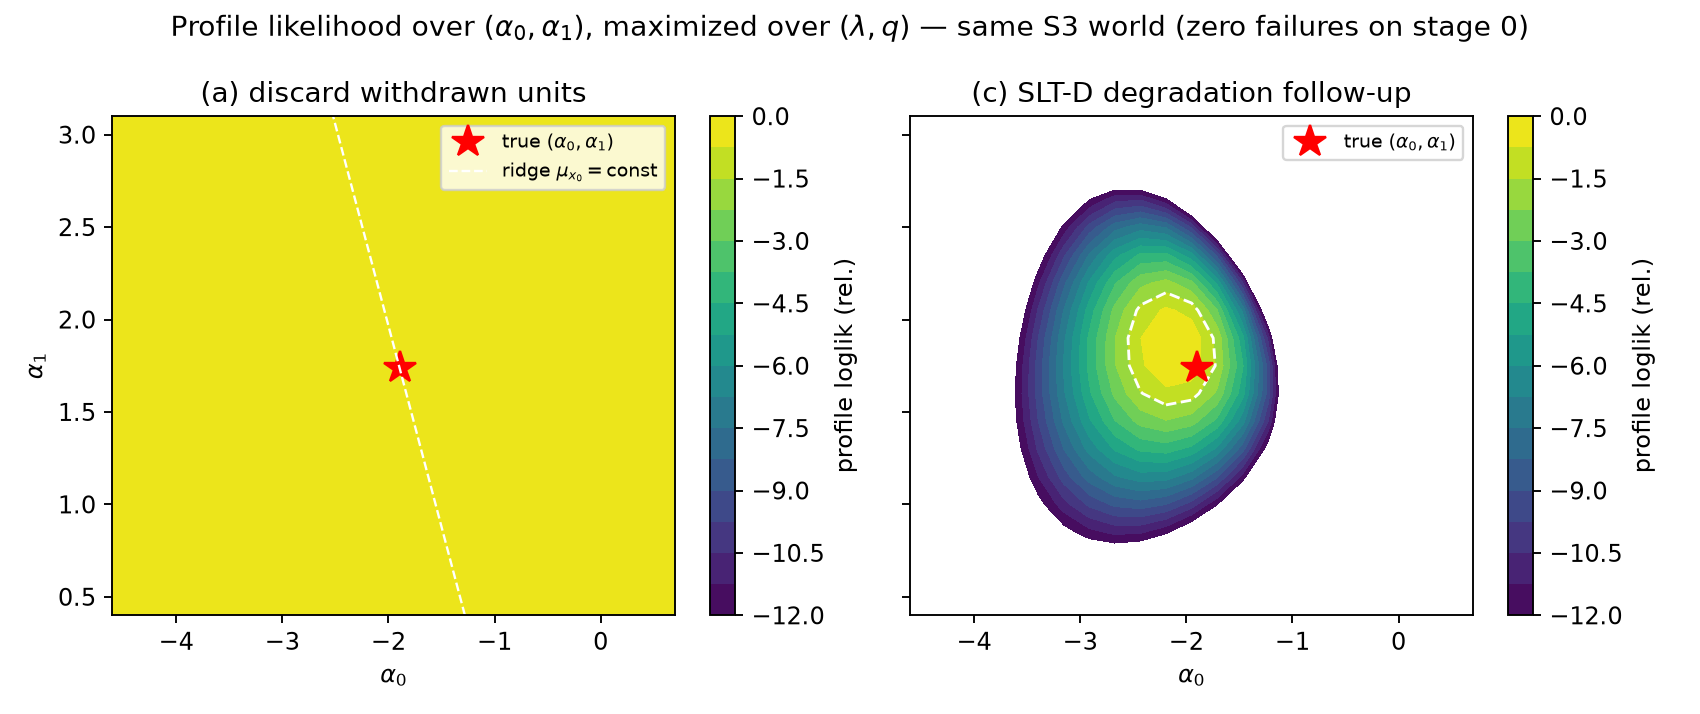
\includegraphics[width=.95\linewidth]{../results/fig3_ridge.png}
\caption{Profile log-likelihood over $(\alpha_0,\alpha_1)$, maximized over $(\lambda,q)$, for
scheme (a) (left) and \SLTD{} (right) on the same realization with zero stage-0 failures (S3).
White contour: approximate 15\% region; the dashed line in the left panel is the
$\mu_{x_0}=\mathrm{const}$ ridge.}
\label{fig:ridge}
\end{figure}

\subsection{Planning formula versus simulated variance}\label{sec:avar}

Table~\ref{tab:avarcheck} compares the planning asymptotic variance \eqref{eq:V} (with the
alive-weighting \eqref{eq:alive}) against the empirical variance of $\ln\hat\xi_{0.1}(0)$ across
the $1000$ replications of \SLTD{}. Agreement is close throughout (S1: $0.66$ vs $0.84$; S2: $0.19$ vs $0.30$; S3: $0.18$ vs $0.19$), supporting the use
of \eqref{eq:I}--\eqref{eq:V} for design optimization. Without the alive-weighting the planning
formula overstates the information substantially whenever withdrawn units fail mid-test (in S2
by about a factor $2.1$ in the dominant eigenvalue; Section~\ref{sec:design}).

\begin{table}[t]
\centering\small
\caption{Predicted planning $\Asvar$ of $\ln\hat\xi_{0.1}(0)$ versus empirical variance across
1000 replications (\SLTD{}, $\pi_1=0.5$).}
\label{tab:avarcheck}
\begin{tabular}{lccc}
\toprule
Design & $n$ & predicted $\Asvar(\log\hat\xi_{0.1})$ & empirical var \\
S1 & 20 & 0.658 & 0.839 \\
S2 & 20 & 0.192 & 0.303 \\
S3 & 30 & 0.175 & 0.194 \\
\bottomrule
\end{tabular}

\end{table}

\subsection{Robustness of the hierarchy to parameter misspecification}\label{sec:sens}

All estimators so far use the true $\theta$ to initialize and all designs were constructed at
the true values. Table~\ref{tab:sensest} repeats the S2 comparison with the \emph{true}
parameters perturbed in an $L_9(3^4)$ array of $\pm10\%$ errors on $(\alpha_0,\alpha_1,\lambda,q)$
(the analysis still being initialized at the unperturbed values, as when planning values come
from a pilot study). The expected number of withdrawn units under the perturbed truth,
$\E[R_1^{*}]=\sum_k\binom{20}{k}F_{x_0}(\tau_1)^k\bar F_{x_0}(\tau_1)^{20-k}\lfloor(20-k)/2\rfloor$,
is shown to expose the mechanism. Three regimes appear. (i) A healthy arm (combinations 1, 5,
6, 7, 9): the hierarchy holds, with \SLTD{} better in RMSE by factors of $1.8$ to $42$. The
largest factor arises in combination 9, where scheme~(b)'s RMSE is dominated by a catastrophic
tail (MdAE $0.32$ against RMSE $15.5$), exactly as at the nominal parameters. (ii) A collapsed
arm (combinations 3 and 4): the perturbed parameters push $\mu_{x_0}$ up so far that
$F_{x_0}(\tau_1)\approx1$; essentially nothing survives to $\tau_1$, both schemes receive
identical stage-0-only data, and both inherit the unidentifiability of
Proposition~\ref{prop:ident} (identical RMSE of about $20$ to $26$). (iii) A thin arm
(combinations 2 and 8): $\E[R_1^{*}]<1$; the stage-0 block again dominates and both schemes
degrade, though scheme~(c)'s median error stays moderate (MdAE $1.8$ to $2.1$).
The lesson here is more about design than about estimation. Near the knee
$a_{x_0}(\tau_1)\approx\omega$ the quantity $F_{x_0}(\tau_1)$ reacts very sensitively to
$\mu_{x_0}$, and the S2 plan sits right there ($a_{x_0}(\tau_1)\approx8.7$ against
$\omega=10$), so a planning error of $\pm10\%$ in $(\alpha_0,\alpha_1)$ swings
$F_{x_0}(\tau_1)$ across most of $(0,1)$. A robust \SLTD{} plan should therefore place
$F_{x_0}(\tau_1)$ well inside $(0,1)$, say between $0.3$ and $0.8$, rather than at the cliff
edge; the plan-level $L_9$ analysis of Section~\ref{sec:design} points the same way, and we
return to this point in Section~\ref{sec:concl}.

\begin{table}[t]
\centering\small
\caption{Estimation robustness: $L_9(3^4)$ array of $\pm10\%$ errors in the true parameters
(S2, 300 replications per combination; errors of $\ln\hat\xi_{0.1}(0)$).}
\label{tab:sensest}
\begin{tabular}{crrrrrrr}
\toprule
Combo & $\E[r_1^*]$ & \multicolumn{3}{c}{scheme (b)} & \multicolumn{3}{c}{scheme (c)} \\
\cmidrule(lr){3-5}\cmidrule(lr){6-8}
 & & Bias & RMSE & MdAE & Bias & RMSE & MdAE \\
1 & 8.8 & 0.132 & 1.205 & 0.608 & -0.038 & 0.420 & 0.267 \\
2 & 0.6 & 3.401 & 11.863 & 1.964 & 3.448 & 11.827 & 1.803 \\
3 & 0.0 & 13.127 & 26.074 & 3.557 & 13.127 & 26.074 & 3.557 \\
4 & 0.0 & 10.961 & 20.139 & 3.803 & 10.989 & 20.144 & 3.811 \\
5 & 9.8 & 0.096 & 0.651 & 0.379 & 0.004 & 0.339 & 0.217 \\
6 & 2.5 & 0.574 & 2.091 & 0.883 & 0.322 & 0.923 & 0.535 \\
7 & 9.8 & 0.053 & 0.497 & 0.324 & -0.016 & 0.274 & 0.187 \\
8 & 0.4 & 5.350 & 13.247 & 2.242 & 5.453 & 13.221 & 2.138 \\
9 & 10.0 & 2.739 & 15.519 & 0.324 & 0.040 & 0.371 & 0.247 \\
\bottomrule
\end{tabular}

\end{table}

\section{Case studies}\label{sec:case}

\subsection{Stress relaxation of electrical connectors}

We use the stress-relaxation data of a type of electrical connector, presented as
Example~8.7 of \citet{Yang2007} and tabulated by \citet{WangWangDuan2016} and \citet{Ma2021}:
Figure~\ref{fig:realdata} shows the 18 observed paths together with the fitted IG mean
degradation $\hat\mu_x\,t^{\hat q}$ at each temperature. The data comprise six units each at
$65$, $85$ and $100^\circ$C, with 10--11 readings per unit over up to 2810 h; failure is
declared at stress relaxation $\omega=30\%$; the Arrhenius standardization gives
$x(65^\circ\mathrm{C})=0.460$, $x(85^\circ\mathrm{C})=0.781$, $x(100^\circ\mathrm{C})=1$. Fitting
\eqref{eq:ig}--\eqref{eq:inc} by maximum likelihood yields
$\hat\theta=(-1.894,\,1.738,\,0.629,\,0.449)$ with $\hat\xi_{0.1}(40^\circ\mathrm{C})=1.20\times
10^{5}$ h, in close agreement with the published estimates
$(-1.88,1.73,0.653,0.449)$ and $1.16\times10^{5}$ h of \citet{Ma2021}. This agreement
validates our likelihood implementation; the remaining differences reflect rounding in the
published table.

\begin{figure}[t]
\centering
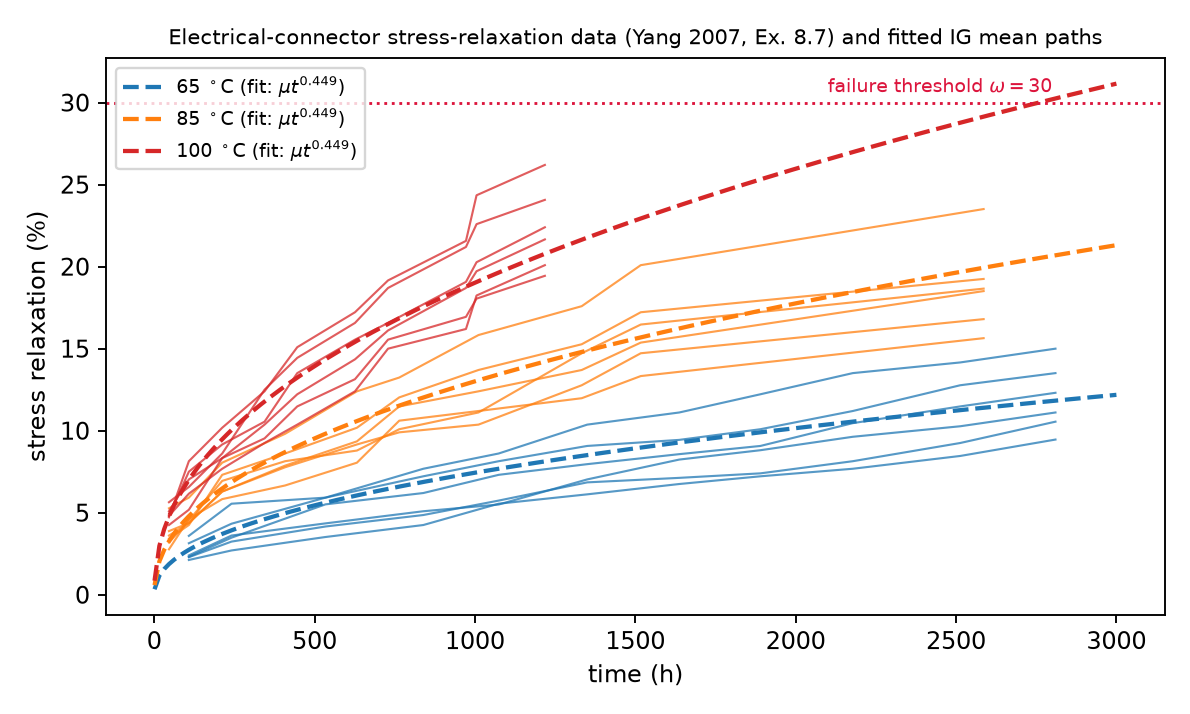
\includegraphics[width=.85\linewidth]{../results/fig_realdata.png}
\caption{Stress-relaxation paths of the 18 connector units (thin lines) and the fitted IG mean
degradation $\hat\mu_x\,t^{\hat q}$ (dashed) at the three test temperatures; the dotted line
is the failure threshold $\omega=30\%$.}
\label{fig:realdata}
\end{figure} Re-using these values as ground truth anchors the simulation study
(Section~\ref{sec:sim}) and the planning analysis (Section~\ref{sec:design}). For this
product, an \SLTD{} with 20 units (a life test at $x_0\approx45^\circ$C for 1750 h, then 90\%
of survivors withdrawn into an $\approx89^\circ$C rig read every 150 h until 5000 h) estimates
the use-condition $0.1$-quantile with a planned relative precision of about $\pm21\%$, and
not a single failure needs to occur.

\subsection{A second product: GaAs laser diodes under unit heterogeneity}\label{sec:laser}

The connector analysis assumed a homogeneous population; real degradation data often violate
this, and the GaAs laser dataset of \citet{MeekerEscobar1998} (p.~339) is a canonical example.
The degradation is the increase of the operating current needed to maintain constant light
output, read every 250 h up to 4000 h for 15 lasers, with failure declared at a 10\% increase
($\omega=10$); three units are observed to cross the threshold
(Figure~\ref{fig:laserdata}). The paths are nearly linear (the homogeneous fit gives
$\hat q = 1.00$ with $\hat\mu = 0.0021$) but strongly heterogeneous across units, with a
per-unit rate CV of about $0.22$. This is why \citet{WangXu2010} and \citet{PengTseng2015}
introduced random-effect extensions of the IG process for these data.

The data allow us to stress the design comparison in a deliberately misspecified setting.
The simulation truth carries the measured heterogeneity (rates $\mu_i$ lognormal with log
standard deviation $0.21$ around the fitted mean $\bar\mu = 0.0021$; $q = 1$; within-unit
dispersion $\lambda = 3\times10^{-5}$), while the estimators remain the homogeneous MLEs that
a practitioner without a random-effect model would fit. The estimand is the
\emph{population} 0.1-quantile of the failure time, $\xi_{0.1}(0) = 3611$ h. Three designs at
the historical resources ($n=15$, $\tmax=4000$ h, 250 h cadence) are compared in
Table~\ref{tab:laser}: the historical full monitoring of all 15 units from $t=0$; an \SLTD{}
that leaves the life test uninstrumented, withdraws 50\% of survivors at $\tau_1=2000$ h into
a rig with Arrhenius acceleration ($E_a = 0.7$~eV between 300~K and 350~K,
$\mathrm{AF}\approx48$); and the pure life test.

The results trace the limits of \SLTD{} (Table~\ref{tab:laser}). All three designs
overestimate $\xi_{0.1}$, by $0.04$ to $0.14$ in log terms; the homogeneous likelihood cannot
represent the mixture, and the observed 3/15 crossings, set against a fitted
$F(4000\,\mathrm{h})\approx0.02$, would flag this immediately in practice. The ranking of
typical accuracy (median error) is more surprising: the pure life test does best ($0.068$),
\SLTD{} comes second ($0.099$), and full degradation monitoring does worst ($0.141$). There
is a simple explanation. The failure/censoring likelihood observes the marginal crossing law,
with the heterogeneity already integrated out. The homogeneous increment likelihood instead
fits pooled increments, which no homogeneous model actually generates, so the additional
degradation information does not translate into better quantile estimates. On robustness,
neither full monitoring nor \SLTD{} produced a degenerate fit in 500 replications, while the
life test did once, and the typical error of \SLTD{} matches that of full monitoring even
though fewer than half of the units are instrumented.

Taken together, the two case studies indicate where \SLTD{} pays off. The gains concentrate
in applications where the first stage runs off the use condition, so that discarding the
withdrawn units is unidentifiable and cross-stress extrapolation is the central inferential
problem, and where unit heterogeneity is mild. When the life test already sits at the use
condition and the units are strongly heterogeneous, the failure/censoring data of the life
test alone are competitive, and random-effect models \citep[cf.][]{PengTseng2015} are the
better investment.

\begin{figure}[t]
\centering
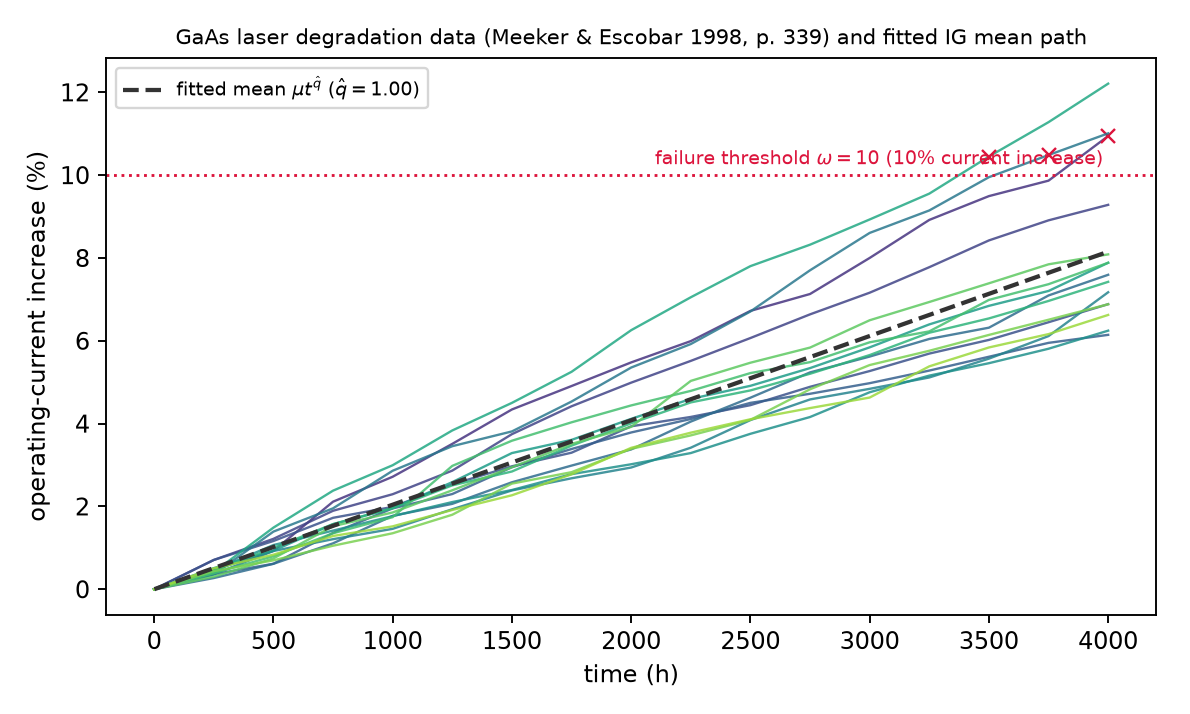
\includegraphics[width=.85\linewidth]{../results/fig_laserdata.png}
\caption{Operating-current increase of the 15 GaAs lasers (Meeker and Escobar
\citeyearpar{MeekerEscobar1998}, p.~339), the fitted homogeneous IG mean path
($\hat q = 1.00$), and the failure threshold $\omega = 10$; crosses mark the three observed
crossings. The spread of the paths at 4000 h (6.1--12.2) visualizes the unit heterogeneity.}
\label{fig:laserdata}
\end{figure}

\begin{table}[t]
\centering\small
\caption{Laser case study: design comparison under data-calibrated heterogeneity
(500 replications; $n=15$, $\tmax=4000$ h, 250 h cadence; errors of
$\ln\hat\xi_{0.1}(0)$ against the population quantile 3611 h).}
\label{tab:laser}
\begin{tabular}{lccrrrr}
\toprule
Design & monitored & degenerate & Bias & RMSE & MdAE & $p_{90}$AE \\
 & units & fits & & & & \\
full monitoring (historical) & 15 from $t{=}0$ & 0/500 & +0.133 & 0.156 & 0.141 & 0.239 \\
\SLTD{} ($\tau_1{=}2000$, $\pi_1{=}0.5$) & $\approx7$ from $\tau_1$ & 0/500 & +0.139 & 0.230 & 0.099 & 0.358 \\
life test only & 0 & 1/500 & +0.042 & 0.193 & 0.068 & 0.216 \\
\bottomrule
\end{tabular}

\end{table}

\section{Conclusions}\label{sec:concl}

Stage life testing posed the question of what the withdrawn units of a progressively
censored life test are worth. Our answer is that, used as degradation-monitoring units, they
are worth a great deal. The \SLTD{} likelihood is exact and available in closed form,
randomized withdrawal makes every block of the data conditionally independent, and discarding
the withdrawn units destroys the stress transfer needed for extrapolation. Failure re-testing
restores identifiability but behaves erratically, while degradation follow-up was uniformly
superior in our simulations. The planning information, refined to account for mid-test
failures of withdrawn units, predicts the simulated precision well and yields V-optimal
plans. Two refinements strengthen the design further. Spreading the withdrawal over several
change times improves precision at a matched number of recycled units and protects the plan
against the survival cliff of a single change time. Bayesian planning under a pilot-informed
prior turns planning-parameter uncertainty into an explicit criterion; for an informative
pilot it certifies the plug-in optimum, and for a weak pilot it fine-tunes that optimum. The
design comparison also states the limits of the proposal. When any unit can be instrumented
from the start and use-condition degradation is readable within the horizon, a parallel
low-stress ADT remains preferable; in the connector case the sequential constraint costs a
factor of about $5.5$ in asymptotic variance. \SLTD{} is the design of choice when the first
stage must be a failure-only test, as in sealed chambers or mandated certification runs, or
when scarce units have to serve both purposes. The laser study adds a boundary condition:
when the life test already sits at the use condition and the units are strongly heterogeneous,
a homogeneous \SLTD{} fit inherits the misspecification bias, the pure life test becomes
competitive, and random-effect models are the more productive route.

Several extensions are worth pursuing: optimal design with Type-M withdrawal and adaptive
change times; Bayesian planning with hierarchical priors elicited from several historical
tests; and random effects across units \citep[cf.][]{PengTseng2015}, which would break the
clean factorization of Lemma~\ref{lem:block} and call for the EM machinery of
Section~\ref{sec:em} at the design stage as well.

\section*{Reproducibility}

All computations are implemented in Python/NumPy/SciPy: the likelihoods, simulators
validated by score identities against the generating model, quadrature checks against Monte
Carlo, the 15{,}000-fit simulation study, and the design optimization. Source code, generated
tables, and figures accompany this manuscript. The GaAs laser data were obtained from the
public repository of Meeker's repeated-measured degradation datasets (file GaAsLaser.csv).

\appendix

\section{First-passage and continuation laws}\label{app:pass}
Equation \eqref{eq:pass} follows from $P(T_x\le t)=P(Y_x(t)\ge\omega)$ and the closed-form IG
survival function $\mathrm{S}_{\mathrm{IG}}(y;a,b)=\Phi\big(\sqrt{b/y}(1-y/a)\big)
-e^{2b/a}\Phi\big(\!-\!\sqrt{b/y}(1+y/a)\big)$; monotonicity of IG paths makes the hitting
event equivalent to the level event, and inversion sampling of $T_x$ is exact. For the
continuation, the path-level CE principle gives virtual age \eqref{eq:w}; the crossing event
by offset $u$ is $\{Y'_{x_1}(w+u)\ge\omega\}$, i.e.\ the continuation increment over $(w,w+u]$
reaching $\omega-b$, which is \eqref{eq:G}; differentiating in $u$ yields $g(u\mid b)$ (computed
by central differences).

\section{Expected information}\label{app:info}
For a single observation $y\sim\mathrm{IG}(a,b)$ with $(a,b)$ functions of $\theta$, the
expected information is $J^{\top}WJ$ with $W=\mathrm{diag}(b/a^{3},\,1/2b^{2})$ and
$J=\partial(a,b)/\partial\theta$: the second-derivative contribution of $\partial J/\partial\theta$
vanishes in expectation because the IG score has zero mean, and
$\E[-\partial^2\ln f/\partial(a,b)^2]=\mathrm{diag}(b/a^3,1/2b^2)$ (verified numerically to
$10^{-2}$ relative error). Summing over the record types of Lemma~\ref{lem:block} with their
probabilities gives \eqref{eq:I}; the alive-weighting \eqref{eq:alive} follows because reading
$j$ is observed iff the unit has not crossed $\omega$ by $u_{j-1}$, an event of probability
$1-G(u_{j-1}\mid b)$ conditionally on the latent (or observed) level $b$, and the crossing
reading itself remains an ordinary IG observation.

\section{EM for the variant without baseline reading}\label{app:em}
With complete data $(b,\Delta_1,\dots,\Delta_L)$ for a withdrawn unit, the complete-data
log-likelihood is the sum of the level log-density at $\tau_1$ and the increment log-densities
of Section~\ref{sec:lik}. The E-step evaluates, by quadrature, the conditional density of $b$
given the observed increments (proportional to the integrand of \eqref{eq:ellB} on
$(0,\min(\ell_1,\omega))$), together with any conditional moments that are needed; the
M-step
maximizes the expected complete-data log-likelihood numerically. Because the increment means
depend on $\theta$ through the virtual age $w(b;\theta)$, the M-step has no closed form, and
direct maximization of the marginal likelihood \eqref{eq:ellB} (used here) is the equivalent
one-step alternative; the observed-data information follows from the numerical Hessian of
\eqref{eq:ellB} (Louis-type corrections are unnecessary at the accuracy required for Wald
intervals).

\begin{thebibliography}{25}

\bibitem[Balakrishnan and Aggarwala(2000)]{BalakrishnanAggarwala2000}
N.~Balakrishnan, R.~Aggarwala, Progressive Censoring: Theory, Methods, and Applications,
Birkh\"auser, Boston, 2000.

\bibitem[Balakrishnan and Cramer(2014)]{BalakrishnanCramer2014}
N.~Balakrishnan, E.~Cramer, The Art of Progressive Censoring: Applications to Reliability and
Quality, Birkh\"auser, New York, 2014.

\bibitem[Doksum and H{\o}yland(1992)]{DoksumHoyland1992}
K.~A. Doksum, A.~H{\o}yland, Models for variable-stress accelerated life testing experiments
based on Wiener processes and the inverse Gaussian distribution, Technometrics 34 (1992)
74--82.

\bibitem[Gouno, Sen, and Balakrishnan(2004)]{Gouno2004}
E.~Gouno, A.~Sen, N.~Balakrishnan, Optimal step-stress test under progressive Type-I censoring,
IEEE Transactions on Reliability 53 (2004) 388--393.

\bibitem[Kundu and Ganguly(2017)]{KunduGanguly2017}
D.~Kundu, A.~Ganguly, Analysis of Step-Stress Models, Academic Press, London, 2017.

\bibitem[Li et~al.(2017)]{Li2017}
X.~Li, Y.~Hu, E.~Zio, R.~Kang, A Bayesian optimal design for accelerated degradation testing
based on the inverse Gaussian process, IEEE Access 5 (2017) 5690--5701.

\bibitem[Laumen and Cramer(2019a)]{LaumenCramer2019}
B.~Laumen, E.~Cramer, Stage life testing, Naval Research Logistics 66 (2019) 632--647.

\bibitem[Laumen and Cramer(2019b)]{LaumenCramer2019pc}
B.~Laumen, E.~Cramer, Progressive censoring with fixed censoring times, Statistics 53 (2019)
569--600.

\bibitem[Laumen and Cramer(2021)]{LaumenCramer2021}
B.~Laumen, E.~Cramer, $k$-step stage life testing, Statistica Neerlandica 75 (2021) 203--233.

\bibitem[Ma et~al.(2021)]{Ma2021}
Z.~Ma, H.~Liao, H.~Ji, S.~Wang, F.~Yin, S.~Nie, Optimal design of hybrid accelerated test based
on the inverse Gaussian process model, Reliability Engineering \& System Safety 210 (2021)
107509.

\bibitem[Meeker and Escobar(1998)]{MeekerEscobar1998}
W.~Q. Meeker, L.~A. Escobar, Statistical Methods for Reliability Data, Wiley, New York, 1998.

\bibitem[Nelson(1980)]{Nelson1980}
W.~Nelson, Accelerated life testing --- step-stress models and data analyses, IEEE Transactions
on Reliability R-29 (1980) 103--108.

\bibitem[Nelson(2004)]{Nelson2004}
W.~B. Nelson, Accelerated Testing: Statistical Models, Test Plans, and Data Analysis, Wiley,
Hoboken, 2004.

\bibitem[Peng and Tseng(2013)]{PengTseng2015}
C.-Y. Peng, S.-T.~B. Tseng, Inverse Gaussian processes with random effects and explanatory
variables for degradation data, Technometrics 55 (2013) 233--248.

\bibitem[Tang et~al.(2025)]{Tang2025}
J.~Tang, et~al., Step-stress accelerated degradation test for inverse Gaussian process,
Scientific Reports 15 (2025) 15171.

\bibitem[Wang, Wang, and Duan(2016)]{WangWangDuan2016}
H.~Wang, G.-J. Wang, F.-J. Duan, Planning of step-stress accelerated degradation test based on
the inverse Gaussian process, Reliability Engineering \& System Safety 154 (2016) 97--105.

\bibitem[Wang and Xu(2010)]{WangXu2010}
X.~Wang, D.~Xu, An inverse Gaussian process model for degradation data, Technometrics 52
(2010) 188--197.

\bibitem[Yan et~al.(2023)]{Yan2023}
W.~Yan, et~al., Optimal design of step-stress accelerated degradation tests using the Tweedie
exponential dispersion process, Reliability Engineering \& System Safety 225 (2023) 108601.

\bibitem[Yang(2007)]{Yang2007}
G.~Yang, Life Cycle Reliability Engineering, Wiley, Hoboken, 2007.

\bibitem[Ye et~al.(2014)]{Ye2014}
Z.-S. Ye, L.-P. Chen, L.-C. Tang, M.~Xie, Accelerated degradation test planning using the
inverse Gaussian process, IEEE Transactions on Reliability 63 (2014) 750--763.

\bibitem[Ye and Chen(2014)]{YeChen2014}
Z.-S. Ye, N.~Chen, The inverse Gaussian process as a degradation model, Technometrics 56
(2014) 302--311.

\end{thebibliography}

\end{document}
